\documentclass[11.5pt]{book}

\usepackage{sectsty, titlesec}
\usepackage{setspace}
\usepackage{wrapfig, rotating, subcaption}
\usepackage{enumitem,tabularx, booktabs}
\usepackage{nomencl}
\makenomenclature
\renewcommand{\nomname}{List of symbols and\\abbreviations}
\usepackage[numbers]{natbib}
\usepackage{graphicx,caption,subcaption}
%\usepackage{cool}  % for pderiv
\usepackage{amsmath, amssymb}
\usepackage{mathspec}
\setmainfont[Mapping=tex-text, Scale=1.1]{Crimson}
\setsansfont[Scale=1]{Alte DIN 1451 Mittelschrift}
%\allsectionsfont{\sffamily}
%\setmainfon
%\usepackage{fouriernc}
%\usepackage[T1]{fontenc}
\newcommand*{\figref}[1]{Fig.~\ref{#1}}
\newcommand*{\secref}[1]{Section~\ref{#1}}
\newcommand*{\chpref}[1]{Chapter~\ref{#1}}
\newcommand*{\tableref}[1]{Table~\ref{#1}}
\setmathsfont(Digits,Latin,Symbols)[Scale=1.1]{Crimson}
\setmathrm[BoldFont={Crimson Bold}, Scale=1.1]{Crimson}
\setmathsfont(Greek)[Scale=1.21]{Crimson}
\newlist{alist}{itemize}{1}
\setlist[alist]{label=---,labelindent=2in,leftmargin=9pt,labelsep=6pt,
itemsep=-1pt}
% Character shortcuts
\newcommand*{\Hhat}{\hat{\vphantom{\scalebox{1.2}{H}} H}}
\newcommand*{\Phat}{\hat{\vphantom{\scalebox{1.2}{P}} P}}

\newcommand*\pderiv[3][]{\frac{\text{\emph{∂}}^{#1} {#2}}{\text{\emph{∂}}
{#3}^{#1}}}
\newcommand*\diff{\mathop{}\!\mathrm{d}}
\newcommand*\Diff[1]{\mathop{}\!\mathrm{d^#1}}
% line spacing
\linespread{1.35}
\usepackage{fancyhdr}
\setlength{\headheight}{15pt}
\setlength{\textwidth}{380pt}
\setlength{\evensidemargin}{54pt}
\setlength{\marginparwidth}{1.2in}
%\titleformat{\section}{\huge\sansnormalfont}{\protect\makebox[0pt][r]{\thesection\quad}}{0em}{}
\titleformat{\chapter}{\fontsize{32pt}{36pt}\selectfont\bfseries}{}{0em}{}
\titleformat{\section}{\fontsize{18pt}{22pt}\selectfont\bfseries}{\protect\makebox[0pt][r]{\thesection\quad}}{0em}{}
\titleformat{\subsection}{\fontsize{12pt}{16pt}\selectfont}{\protect\makebox[0pt][r]{\thesubsection\fontsize{18pt}{22pt}\selectfont\quad}}{0em}{}
%\titleformat{\paragraph}{\fontsize{12pt}{16pt}\selectfont}{}{}{}
\pagestyle{fancy}
\renewcommand{\chaptermark}[1]{ \markboth{#1}{} }
\renewcommand{\sectionmark}[1]{ \markright{#1}{} }

\fancyhf{}
\fancyhead[LE,RO]{\sffamily\thepage}
\fancyhead[RE]{\sffamily{ \nouppercase{\leftmark}} }
\fancyhead[LO]{\sffamily{ \nouppercase{\rightmark}} }

\fancypagestyle{plain}{ %
  \fancyhf{} % remove everything
  \renewcommand{\headrulewidth}{0pt} % remove lines as well
  \renewcommand{\footrulewidth}{0pt}
}

\parskip 0pt
%\usepackage{xunicode}
\begin{document}
\title{Calibration of ILIDS and PDPA droplet sizing systems and their
application to the breakup of impacting water and air jets}
\author{Sebastian Kosch, University of Toronto}
\date{2015}
\maketitle

\printnomenclature[5em]

\chapter{Introduction}
\section{Why spray sizing is important}

Fluid sprays find application in numerous designs, ranging from fuel injection
and coating systems to medical and printing devices. Often, the droplet size is
a major factor in how well these systems perform. Consequently, measuring the
characteristics of a given spray to a useful degree of accuracy is an important
task with relevance to several areas of mechanical engineering.

Due to the behaviour and size of the droplets in typical sprays, only
non-intrusive instrumentation methods come into question. The most popular
techniques rely on illumination of the spray with laser light. The droplets
scatter the light, and it is picked up by a set of detectors, such as
photomultiplier tubes or digital cameras. Depending on the position of the
detectors, the motion of the droplets, their size, and the laser light's known
properties, the detected patterns can be processed to yield information about
the spray's characteristics.

While countless different optical setups are in use in laboratories the world
over, all of them rely on the same fundamental optical principles governing the
scattering of light. This paper aims to offer a high-level derivation of these
principles.

\section{What our contributions in this paper are}
- Our contributions:
    - Pupillary magnification has to be taken into account
    - Circle detection algorithm is crap
\section{What other work has been done in this area}

\chapter{Experimental setup}
- What kinds of setups there are

- Our setup:
\section{Dantec system}
    - Dantec system
\section{PDPA system}
    - TSI system

\chapter{Mie scattering}
In this chapter, we will discuss some of the fundamentals of Mie scattering.
The majority of the equations and derivations herein are adapted directly from
\citet{Albrecht03}.
For the purposes of this discussion, we will model light as a coupled pair of
electrical and magnetic fields, $\bf{E}$ and $\bf{B}$, which at every point in
space obey Maxwell's equations
\begin{align}
    \nabla \cdot \bf{E} &= \frac{\rho}{\epsilon_0}\\
    \nabla \cdot \bf{B} &= 0 \\
    \nabla \times \bf{E} &= -\pderiv{\bf{B}}{t} \\
    \nabla \times \bf{B} &= \mu_0 \sigma {\bf E} + \mu_0 \epsilon_0
    \pderiv{\mathbf{E}}{t},
\end{align}
where the constants $\epsilon_0$ and $\mu_0$ represent the electric permittivity
and magnetic permeability in vacuum, respectively; $\rho$ is the local charge
density, and $\sigma$ is the electric conductivity (such that $\sigma \bf{E} =
\bf{J}$ is the current density).

Electromagnetic radiation propagates in a direction $\bf{S}$ orthogonal to the
planes of oscillation of $\bf{E}$ and $\bf{B}$, which are themselves orthogonal
to one antoher:
\begin{equation}
    {\bf S} = \mathbf{E} \times \mathbf{B}.
\end{equation}
$\mathbf{S}$ is called the \emph{Poynting vector}.

Note that this definition leaves $\mathbf{S}$ invariant to a rotation of
$\mathbf{E}$ and $\mathbf{B}$ around $\mathbf{S}$. The rotation angle is called
\emph{polarization} and need not be constant along the line of propagation
(``circular polarization''), although we will here assume that it is (``linear
polarization'') to simplify our derivations. This assumption is justified in
typical spray characterization applications, for gas lasers use \emph{Brewster
windows} both as mirrors and output windows which act as polarization filters.

We will also assume here that $\mathbf{S}$ is approximately constant over the
surface of the droplet. In other words, we assume the incoming light wave to be
plane. Whether this is a reasonable assumption depends on the configuration of
the laser optics, on the width of the laser beams and on the size of the
droplet. We will see in Section \ref{sec:mietheory} that more complex models
without this assumption can be used, but they are not suitable for showcasing
the fundamental concepts behind droplet light scattering.  Finally, we assume
the droplet in question to be perfectly spherical.

\subsection{Scattering phenomena}

When light hits a spherical, transparent droplet, three phenomena can be
observed:
\begin{enumerate}
    \item Diffraction
    \item Reflection
    \item Refraction
\end{enumerate}
We will consider each one in this paper, and derive its influence on the
scattered field.

In the following discussion, we will use a coordinate system centered on the
droplet. Let the $z$-axis be aligned with the direction of the plane wave
incident on the droplet, and define the rotation of the $x$-$y$-plane to be at an
arbitrary but fixed angle with respect to light source and detector. Consider
then an infinitesimally small light ray scattered by the droplet. We shall
designate the direction of the scattered ray to be at a deviation angle $\phi$ with
respect to the $x$-axis, and to be at a deviation angle $\vartheta$ with respect
to the $z$-axis.

We also define the plane between the scattered direction and the scattered
direction's projection onto the $x$-$y$-plane as the \emph{scattering plane}. This
allows us to treat any incident polarization as a linear combination of
polarization parallel to that scattering plane ($\vartheta$-field) and
perpendicular to it ($\phi$-field). 

\section{Diffraction} Diffraction, sometimes described as the ``bending'' of
light waves, is the phenomenon observed when plane waves -- even material waves
-- encounter the edge of an obstacle and spread out spherically behind it. While
most of the scattered intensity is focussed along the original wave path, the
scattered fields from two or more edges will interfere behind the obstacle and
create an intensity pattern dependent on both the wavelength and the edges'
separation.

%\begin{figure}
%\centering
%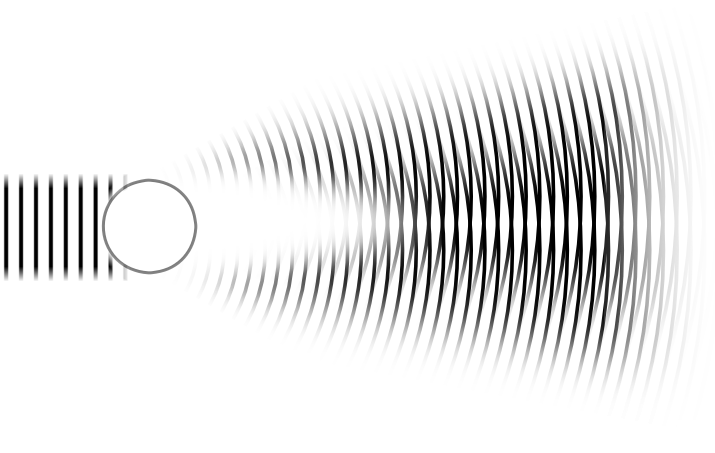
\includegraphics[width=0.6\textwidth]{pictures/diffraction.jpg}
%\caption{Diffraction \cite{orbs}}
%\label{fig:diffraction}
%\end{figure}

A droplet in a plane wave, just like a hole of the same size, has one circular
edge (or a set of infinitely many point-sized edges arranged in a circle). The
diffracted fields interfere behind the particle, as shown in Figure
\ref{fig:diffraction}, to form a periodic intensity pattern.

The viability of exploiting diffraction as a spray characterization principle is
limited, because the phenomenon is strongest when droplet sizes are close to the
light's wavelength. We will thus focus here on scattering phenomena relevant to
techniques such as \emph{Phase Doppler Anemometry} and \emph{Interferometric
Particle Imaging}.

\section{Reflection and refraction}
Detectors used in spray diagnostics are ultimately based on the photoelectric
effect, and thus sensitive only to incident light intensity. This is the case
both for \textsc{CMOS} or \textsc{CCD} cameras used in interferometric
techniques and for photovoltaic cascade amplifiers commonly used in Phase
Doppler setups. As a result, we are interested in accurately modelling the light
intensity at a location $\langle \phi, \vartheta, z \rangle$.

A general description of the scattering process would trace a ray of light
through the droplet. At every encounter with an interface
(air$\rightarrow$water, or water$\rightarrow$air inside the droplet), some of
the light is \emph{reflected off} the interface and some is \emph{refracted
through} the interface. When first incident, the refracted light ray is cast
\emph{into} the droplet; subsequent scattering events will refract some light
\emph{out} of the droplet while the remainder continues scattering within the
droplet until all energy is refracted out or absorbed as heat. Scattering events
are enumerated; the \emph{scattering order} $N$ refers to the
$N$\textsuperscript{th} reflection/refraction.

Total intensity at any location is a function both of the intensity of all
infinitesimal light rays scattered onto that location, but also of the phases of
those light rays, as two equally intense light rays will extinguish one another
if they are in opposite phases. We will thus derive expressions for both
intensity and phase of infinitesimal light rays scattered through the droplet.

\subsection{Intensity from interface separation}
Consider an infinitesimal ray incident, at an angle $\theta_i$, on the surface
of the droplet. We are interested in the respective proportions of light
reflected and refracted.

Following the continuity requirement for components of $\mathbf{E}$ and
$\mathbf{B}$ parallel and perpendicular to the droplet's interface (depending on
the polarization component), and the conservation of energy, we can arrive at
\emph{Fresnel equations:}
\begin{align}
    \label{eq:fresnelequations}
    &r_\vartheta = \frac{m \cos \theta_i - \cos \theta_t}{m \cos \theta_i +
\cos \theta_t},\quad
r_\phi = \frac{\cos \theta_i - m \cos \theta_t}{\cos \theta_i +
m \cos \theta_t}
\end{align}
with $\theta_t = \arcsin\left(\frac{\sin \theta_i}{m}\right)$, and $m$ the
relative refractive index of droplet and medium (e.g. $m = 1.33/1.0$ for the
water$\rightarrow$air transition).

Squaring these numbers yields a reflectance coefficient $R = |r|^2$ for both
polarization directions, and since $R + T = 1$, the computation of $T$ is
then trivial.

\subsection{Intensity from geometry}
An infinitesimal plane wave ray incident on a curved surface will inevitably
experience deviation into a diverging ray (convex surface) or a converging ray
(concave surface).

\begin{figure}
\centering
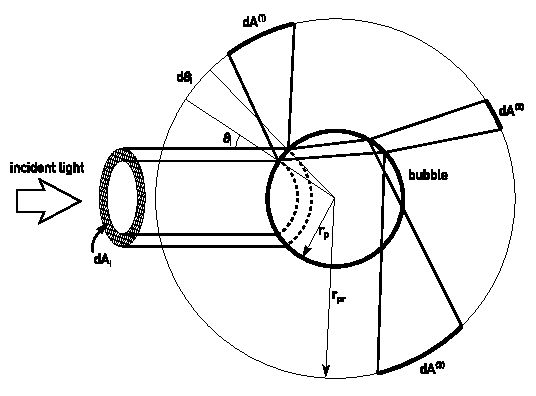
\includegraphics[width=0.75\textwidth]{img/scattering/scatterintensity.pdf}
\caption{Ray divergence due to curved interfaces. Note that here a bubble in
water is used instead of a droplet. Adapted from \citet{Albrecht03}}
\label{fig:scatterintensity}
\end{figure}

Consider Figure \ref{fig:scatterintensity}. An annular ray of surface area
$\diff A_i$ is incident on the droplet of radius $r_p$. The first-order scattering is shown: the
infinitesimal thickness of the ray results in an annular illuminated surface
region between the angles $\theta_i$ and $\theta_i + \diff \theta_i$ of area
\begin{equation}
   \diff A_i = \pi r_p^2 \sin(2 \theta_i + \diff \theta_i) \sin(\diff \theta_i)
\end{equation}
The reflected portion of the light diverges; its cross-section has a
divergence angle of $2\diff \theta_i$.

We can now imagine a sphere around the droplet. Its radius equals the distance
to the detector, $r_{pr}$. The area of that sphere illuminated by the reflected
portion of $\diff A_i$ can be geometrically shown to be
\begin{equation}
    \diff A^{(1)} = 4\pi r_{pr}^2 \sin(2\theta_i + \diff \theta_i)\sin(\diff
    \theta_i).
\end{equation}
The ratio between them is then
\begin{equation}
    \label{eq:intensitydivergence}
    I_r^{(1)} = \frac{\diff A_i}{\diff A^{(1)}} = I_w \frac{r_p^2}{4r_{pr}^2}.
\end{equation}
The ratio $r^2_p / r^2_{rp}$ varies based on the setup; to normalize it we
place a point source of the same intensity of light at the centre of the
droplet and consider its intensity at $r^2_p$:
\begin{equation}
    I_P = I_w\frac{r^2_p}{r^2_{pr}}
\end{equation}
We drop this term from equation \eqref{eq:intensitydivergence} and arrive at a
fixed fraction, or \emph{gain factor}, of $G^{(1)} = \frac{1}{4}$. This number
represents the ``dilution of energy'' associated with the divergence inherent in
reflection off a curved surface.

Similar gain factors can be derived for any other scattering order $N$ of light
leaving the droplet:
\begin{equation}
    \label{eq:gainfactor}
    G^{(N)} = \left| \frac{\sin \theta_i \cos \theta_i}{\sin D^{(N)}} \left(2
    \frac{(N-1)\cos \theta_i}{m \cos \theta_t} - 2\right)^{-1} \right|
\end{equation}
with
\begin{equation}
    D^{(N)} = 2(N-1) \arcsin \left(\frac{\sin \theta_i}{m}\right) - (N-2)\pi -
    2\theta_i.
\end{equation}

\subsection{Path-length differences}
Whether light rays interfere constructively or destructively depends on the
phase difference between them. Since all rays are generated in phase in the
laser cavity, possible phase differences must be due to path length differences,
distortion of the wave (focal shift) or reflection effects. We shall first
discuss the treatment of path lengths.

To effectively compare path lengths between various rays, it is practical to
establish a reference path length for common comparison. This reference ray is
typically pictured as passing through the center of the droplet -- an optical
anomaly as it were, but geometrically useful.

\begin{figure}
\centering
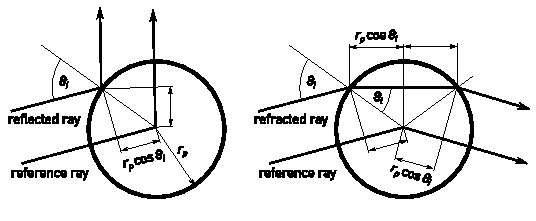
\includegraphics[width=0.9\textwidth]{img/scattering/pathlength.pdf}
\caption{Path length differences, adapted from \citet{Albrecht03}}
\label{fig:pathlength}
\end{figure}

A ray incident at an angle $\theta_i$ and reflected off the surface of the
particle then has a path length $2kr_p \cos \theta_i$ shorter than that of the
reference ray, where $k$ is the wave number of the light ray. This situation is
illustrated in Figure \ref{fig:pathlength}a.

A more general equation for phase length difference is
\begin{equation}
    \varphi^{(N)} = 2kr_p(\cos \theta_i - (N-1)m \cos \theta_i),
\end{equation}
where $\varphi$ stands for the phase difference and is not to be confused with
the scattering plane's orientation $\phi$.

\subsection{Phase shifts at reflection}
A ray's phase is further affected upon reflection. This relationship is quite
complex and depends on the critical and Brewster angles between the two media,
the polarization angle and the relative refractive index. For example, the phase
is flipped when a ray is reflected off a medium with higher refractive index
(such as a water droplet), if the ray is polarized parallel to the interface and
the incident angle does not exceed the Brewster angle. Similar relationships
hold for all other conditions.

The derivations of these phase change formulae follow from the Fresnel equations
\eqref{eq:fresnelequations} shown above and from the understanding that incident
and refracted amplitudes must always sum to the refracted amplitude (which is
zero for total reflection), i.e. continuity of amplitudes across interfaces.
They are widely published (e.g. \citet{Hecht02}) and algebraically
straightforward but lengthy, and thus not included here.

\subsection{Phase shifts through focussing}
While the phase of a plane wave ray does not change (except for the wave's propagation
through time and space), the phase of a diverging or converging ray is affected
by the angle determining the ray width change as follows:
\begin{equation}
    \varphi^{(N)} = \pi \left( (N-1) - \frac{1}{2}\left[1 +
    \mathrm{sgn}\left(\pderiv{D^{(N)}}{\theta}\right)\right]\right),
\end{equation}
The derivation given in \citet{Vandehulst12} explains this as a phase
shift of $\pi/2$ whenever an astigmatic ray passes a focal line.

\subsection{Scattering functions}
The expressions given in the above sections can be combined into
\emph{scattering functions} for both polarization directions as follows:
\begin{equation}
    S_1^{(N)} = \sqrt{i_\phi^{(N)}} \exp(j \varphi_\phi^{(N)}), \quad S_2 =
    \sqrt{i_\vartheta^{(N)}} \exp(j \varphi_\vartheta^{(N)}).
\end{equation}
Here, $i$ is the intensity coefficient
\begin{equation}
    i_{\vartheta,\phi}^{(N)}(\lambda, d_p, m, \theta_i) = \left(\frac{\pi
    d_p}{\lambda}\right)^2 \alpha^{(N)}_{\vartheta,\phi} G^{(N)}
\end{equation}
defined in terms of wavelength $\lambda$, droplet
diameter $d_p$, gain factor $G^{(N)}$ as given in \eqref{eq:gainfactor} above, and
$\alpha^{(N)}$, which is a shorthand for the product of all applicable
reflectance and transmittance coefficients:
\begin{equation}
    \alpha^{(N)}_{\vartheta,\phi} = \begin{cases} R_{\vartheta,\phi}, & N=1
    \\[2ex]
R_{\vartheta,\phi}^{N-2} T_{\vartheta,\phi}^2, & N \geq 2 \end{cases}.
\end{equation}
The $\exp(j \varphi_{\phi,\vartheta}^{(N)})$ terms represent the phase shift
added to the wave function term in \eqref{eq:fulltransfer}

We can use these two-component scattering functions to write a full expression
relating the incident light wave $\mathbf{E}_i$ in its components $\langle E_{ix},
E_{iy} \rangle$ to the wave received by the detector, $\mathbf{E}_r$:

\begin{align}
    \label{eq:fulltransfer}
    {\bf E}_r = &\frac{\exp(-j k r_{pr})}{k r_{pr}}
    \left[ \begin{array}{c c}\cos \beta_{\vartheta x} & \cos \beta_{\phi x} \\
            \cos \beta_{\vartheta y} & \cos \beta_{\phi y} \end{array} \right]
    \\
    &\left[ \begin{array}{c c} \sum_{N=0}^{\infty} S_1^{(N)} & 0 \\
    0 & \sum_{N=0}^{\infty} S_2^{(N)}
  \end{array} \right] \times
\left[ \begin{array}{c c} -\sin \phi & \cos \phi \\ \cos \phi & \sin \phi \end{array} \right]
\left[ \begin{array}{c} E_{ix} \\ E_{iy} \end{array} \right]
\end{align}

The first term evaluates to a sinusoid function corresponding to the scalar
component of the light wave. The second term (and first matrix) represents the
geometrical relationship between the light source and the detector, expressed in
terms of the off-angle $\beta$. Similarly, the matrix in $\phi$ represents the
angle between light source and droplet. By multiplying the $\beta$ matrix with
the appropriate scattering functions (which are summed over all scattering
orders $N$), we arrive at the correct intensity at the detector's location.

\section{Mie theory}
The above derivations, commonly termed \emph{geometrical
optics}, are physically intuitive and therefore useful in the understanding and
design of measurement instrumentation. Geometrical optics, however, are limited
to incident waves that are both plane and much smaller in wavelength than the
droplet diameter. A more general approach is therefore desirable for carrying
out detailed numerical simulations.

Such a numerical system was developed independently by Ludvig Lorenz and Gustav
Mie based on analytical solutions presented here briefly. The Mie scattering
theory decomposes the incoming light into an infinite series of not plane, but
spherical waves concentrical with the droplet. The spherical waves are not
uniform; their dependence depends on the angle $\theta$.

The derivation in scalar terms assumes a scalar field magnitude $\psi$ that solves
\begin{equation}
    \nabla^2 \psi + k_m^2 \psi = 0
\end{equation}
where $k_m^2$ is the magnitude of the field in the surrounding medium.

In spherical coordinates, this leads to
\begin{equation}
    \frac{1}{r^2}\pderiv{}{r}(r^2 \pderiv{\psi}{r}) + \frac{1}{r^2 \sin \theta}
    \pderiv{}{\theta}    (\sin \theta
    \pderiv{\psi}{\theta}) + \frac{1}{r^2 \sin^2 \theta}
    \pderiv[2]{\psi}{\psi} + k^2_m \psi = 0
\end{equation}
Which is solved by
\begin{equation}
    \psi (r, \theta, \phi) = R(r) \Theta (\theta) \exp (\pm i m \phi)
\end{equation}
according to \citet{Ng00}.

Solving for the function governing angular dependence, $\Theta(\theta)$, leads
to Legendre polynomials. Polar plots of the first five such functions of
both types are shown in Figure \ref{fig:angularfuncs}. 

%\begin{figure}
%    \centering
%    \includegraphics[height=0.6\textheight]{pictures/angularfuncs.jpg}
%    \caption{Associated Legendre polynomials. Incident light is coming from the
%    left. Plot by Bohren and Huffman \cite{craig}}
%    \label{fig:angularfuncs}
%\end{figure}

Solving for $R(r)$, the function describing the intensity of the spherical waves
as it drops with distance from the droplet, leads to vector spherical harmonics.
Two-dimensional plots of a few orders of such ``Riccati-Bessel functions'' are
shown in Figure \ref{fig:besselfuncs}.

%\begin{figure}
%    \centering
%    \includegraphics[height=0.8\textheight]{pictures/besselfuncs.jpg}
%    \caption{Riccati-Bessel functions governing the radial decay of the partial
%    waves. Plot by Bohren and Huffman \cite{craig}}
%    \label{fig:besselfuncs}
%\end{figure}

Each partial wave, in turn, represents the sum of scattering effects up to some
scattering order $N$ (in practice, no infinite sum can be taken; the maximum
scattering order to achieve negligible errors depends on the relative
wavelength). With every refraction out of the droplet -- thus adding to the
total external field -- the \emph{internal} partial wave loses intensity
according to respective reflectance and transmittance values. This concept is
illustrated in Figure \ref{fig:miewaves}.

%\begin{figure}
%    \centering
%    \includegraphics[height=0.3\textheight]{pictures/miewaves.jpg}
%    \caption{Schematic illustration of wave series. By Albrecht et al.
%    \cite{albrecht}}
%    \label{fig:miewaves}
%\end{figure}

The complete model, then, provides a semi-closed expression for the scattering
functions $S_1$ and $S_2$:
   \begin{align}
      S_1(\vartheta) &= \sum_{n=1}^{\infty} a_n\pi_n(\vartheta) +
      b_n\tau_n(\vartheta) \\
      S_2(\vartheta) &= \sum_{n=1}^{\infty} a_n\tau_n(\vartheta) +
      b_n\pi_n(\vartheta) \\
      a_n &= \frac{2n+1}{2n(n+1)} (1-R^{MM}_{a_n} - \sum_{p=2}^{\infty}
      T_{a_n}^{MP} (R_{a_n}^{PP})^{p-2} T_{a_n}^{PM}) \\
      b_n &= \frac{2n+1}{2n(n+1)} (1-R^{MM}_{b_n} - \sum_{p=2}^{\infty}
      T_{b_n}^{MP} (R_{b_n}^{PP})^{p-2} T_{b_n}^{PM}) \\
      \mathrm{e.g.\;} R_{b_n}^{PP} &= \frac{\zeta_n(m \frac{\pi
      d_p}{\lambda})\zeta_n'(\frac{\pi d_p}{\lambda}) -
      m\zeta_n(\frac{\pi d_p}{\lambda})\zeta_n'(m \frac{\pi
      d_p}{\lambda})}{-\frac{\pi d_p}{\lambda}\xi_n(m \frac{\pi
      d_p}{\lambda})\zeta'(\frac{\pi d_p}{\lambda}) + m\zeta_n(\frac{\pi
      d_p}{\lambda})\frac{\pi d_p}{\lambda}\xi'(m \frac{\pi
      d_p}{\lambda})}
    \end{align}
    where $PP$ stands for interal reflection, $MM$ external reflection, and $MP$
    and $PM$ for refraction into and out of the particle, respectively. The
    expression for $R_{b_n}^{PP}$ is shown above to illustrate the coefficents'
    form. Note that $\pi$ and $\tau$ are the associated Legendre functions
    shown in Figure \ref{fig:angularfuncs}, and $\zeta$ and $\xi$ are the Riccati-Bessel functions shown in
    Figure \ref{fig:besselfuncs}.

    \subsection{Results}
    Some numerical results are presented in Figures \ref{fig:angleresults} and
    \ref{fig:results} below. The former shows logarithmic and linear plots of the
    total external intensity depending on the droplet size/wavelength ratio. The
    latter shows the angular dependence of various scattering orders for both
    parallel and perpendicular polarizations.

\chapter[Monodisperse droplet generation]{Monodisperse\\droplet generation}
\label{sec:droplet-generator}

To calibrate any droplet sizing device, we need droplets of known and uniform
size. Sprays or streams of such uniform droplets are called \emph{monodisperse},
and many different varying approaches to generating them have been proposed,
each one with advantages and drawbacks.

The most basic type of droplet generator is a capillary tube, for instance a
hypodermic needle or a pulled glass pipette. Droplets are generated as the
liquid flows through the tube due to its own weight. As the liquid leaves the
tube, it wets the tip of the tube and forms a bead held together by surface
tension. Eventually, the bead's gravitational forces overcome the attraction to
the tube surface, and the drop separates from the tube.

Given a liquid and its physical properties, the only remaining controllable
variable is the diameter of the capillary tube tip. As a rule, droplets
generated in this fashion will be significantly larger than the tube diameter
from which they grow. Most droplet generators are designed to prevent this from
happening:
\begin{alist}
\item \emph{Aerodynamic} droplet generators use coaxial air flow to shear the
    forming droplet off of the capillary tip before it can grow to full size.
\item \emph{On-demand} droplet generators use a pressure pulse to eject a fixed
    amount of liquid out of the capillary (or other orifice).
\item \emph{Continuous-stream} droplet generators use mechanical vibrations to
    break up a continuous jet of liquid emanating from the capillary into
    monodisperse droplets.
\end{alist}
More exotic types of droplet generators exist: \citet{Walton49} suggested that
water falling on spinning disks is propelled outwards, forming nearly
monodisperse droplets, and several improved designs have been published since.
Another approach, e.g. used by \citet{Merritt77}, involves mechanized dipping of
a needle into a liquid reservoir, and then flicking it so as to produce one
droplet.

\section{Aerodynamic droplet generators}
\citet{Allan88} provide a history of aerodynamic designs: the first design was
published in 1947 by \citet{Lane47}; \citet{Reil69} later improved on it by
using time-controlled air pulses instead of a continous flow. Coggins and Baker
\cite{Coggins83} have proposed a more elaborate apparatus with variable air and liquid
flow and adjustable needle position.

\subsection{Stry design}
Initial tests based on a design by \citet{Stry92} showed that the ability of the
instrument to produce droplets below 600$\,\mu$m depends entirely on the
precision with which the flow of water and air can be controlled.
\begin{figure}
\centering
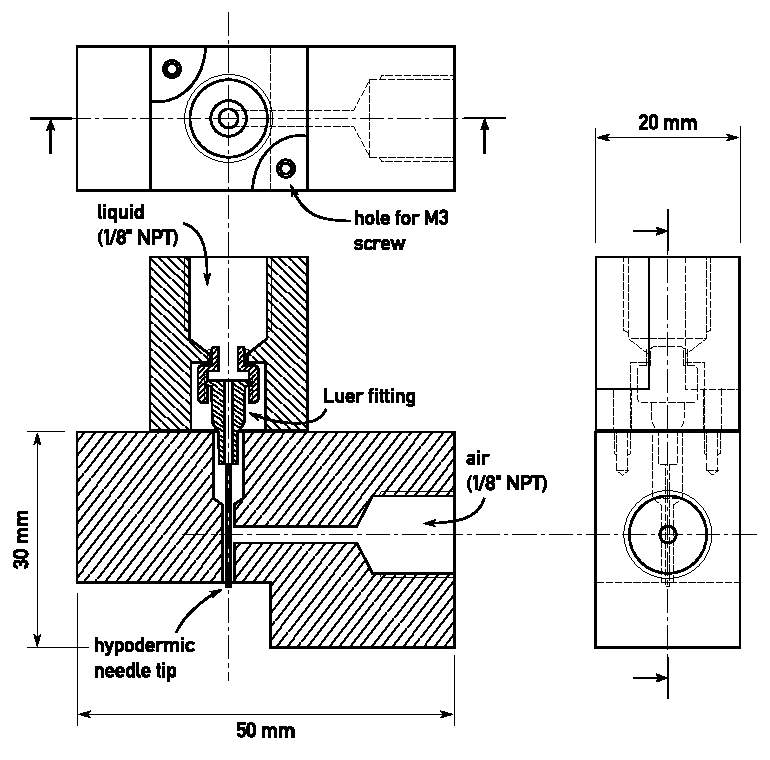
\includegraphics[width=\textwidth]{img/setup/stry.pdf}
\caption{Schematic drawing of the coaxial-flow aerodynamic droplet generator,
based on \citet{Stry92}. Top: top view, right: rear view (third angle
projection). Sectional view illustrates operating principle.\label{fig:stry}}
\end{figure}

\section{On-demand drop generators}
Drop-on-demand technology finds its most important application in printing.
Indeed, the most prominent designs representative of this category are the thermal droplet
generators found in most household inkjet printers, invented by \citet{Endo88}.
At least one research group, \citet{Sergeyev06}, has succeeded in repurposing
an old inkjet print head for laboratory droplet generation.

Less widespread, but more flexible in a research setting, are on-demand
generators driven by the contraction of piezoelectric elements, such as those
proposed by \citet{Yang97} or \citet{Ulmke99}. Excellent reviews on
drop-on-demand designs were published by Le and Lee \cite{Le98, Lee02}. 

A curious third type of on-demand generator by \citet{Goghari08} uses a short
pulse of pressurized air, controlled by a solenoid valve, to eject a small
amount of liquid through an orifice.

While drop-on-demand generators are a crucial component in applications like inkjet
printing or microfluidics, they tend to suffer from aspired air bubbles, pileup
of liquid around the nozzle tip, clogging, and other issues thwarting reliable
drop expulsion unless manufactured and operated with great attention to detail.

\subsection{Amirzadeh Goghari and Chandra design}
We constructed a droplet generator based on the design by \citet{Goghari08}.
While both its construction from off-the-shelf parts and its operation are
remarkably straightforward, it has two limitations:

\begin{alist}
    \item the duration of the air pulse is limited by the response time of the
        solenoid valve used. The shortest pulse we were able to reliable produce
        was on the order of a few milliseconds, which did not permit us to
        produce droplets smaller than a few hundred microns in diameter, and
    \item the head of water over the orifice must be kept very low to prevent 
        leakage. As a result, the number of droplets that can be ejected is
        limited before the water needs to be replenished.
\end{alist}

Owed to our lack of access to an automatic micropipette puller, the nozzles used
in this experiment were not optimal, which likely contributed to our experience
of frequent satellite droplets and liquid buildup at the nozzle tip.

\subsection{Modified Yang design}
A popular piezoelectric-based drop-on-demand design was proposed by
\citet{Yang97}. It consists of a liquid-filled chamber, one wall of which is the
underside of a piezoelectric disk---a brass disk coated with a circular piece of
piezoelectric material, commonly found in electric buzzers.

To evaluate the performance of such a drop generator, we constructed several
modifications of it, the final one of which is shown in \figref{fig:flatyang}.
To make the chamber as flat as possible, minimizing the distance between
piezoelectric disk and orifice, it has a depth of only about 2.5$\,$mm, the
thickness of a sheet of acrylic. A second sheet holds the disk in place, while a
third sheet makes up the bottom wall of the chamber. Nozzle and inlet are glued
directly into the bottom sheet.

To operate the droplet generator, water is fed through
the inlet port until the chamber is filled and all air bubbles have escaped
through the upward-facing nozzle. The generator is then turned so that the nozzle
faces down and $30\,$ms pulses of about $30\,$V are delivered to the
piezoelectric disk.

The greatest challenge faced was the accumulation of liquid on the nozzle
surface, which quickly led to satellite droplets or thwarted droplet production
altogether.  % TODO: add detail about the different nozzle types we tried

Again, capillaries drawn with an automatic pipette puller are likely
more resistant to this effect.

\begin{figure}
\centering
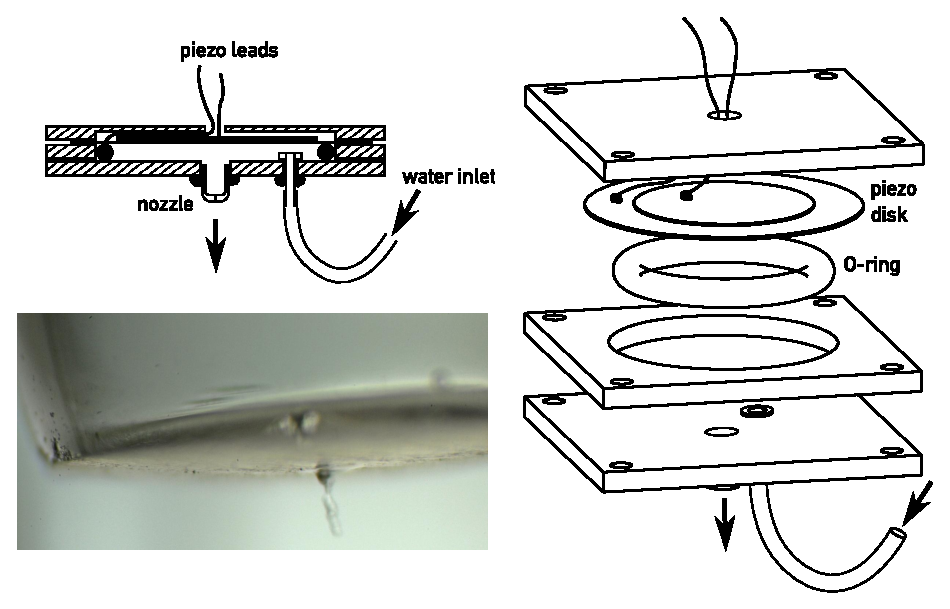
\includegraphics[width=\textwidth]{img/setup/flatyang_exploded.pdf}
\caption{Top and right: schematic cross-section and exploded view of our
    piezoelectric droplet generator. Bottom left: photomicrograph of the nozzle
    tip ejecting a column of water (diameter $\approx 125\,\mu$m), which is about to coalesce into a
round droplet. \label{fig:flatyang}}
\end{figure}

\subsection{Piezo-based drop generator}
We tried building a Piezodropper from old piezoelectric elements squeezing glass
capillaries (just like in the Ulmke paper), but two of the piezo elements were
broken, and the third one had a capillary that clogged up repeatedly. We
abandoned the approach before building a functioning droplet generator, although
it seems attractive in practice. One downside is that the generation of
amplified signals isn't straightforward -- we used a soundcard connected to an
amplifier to generate the signals.

\section{Continuous-stream drop generation}
There exist continuous-stream drop generators based on coaxial air flow
\cite{Green89} and on,
but most continuous-stream drop generators are based on
\emph{Rayleigh breakup}, i.e. the disintegration of a disturbed liquid jet into
droplets. The physics behind this phenomenon have been studied for almost two
centuries \cite{Savart33, Rayleigh79} and are well-understood. When the jet
disturbances are induced by carefully controlled mechanical vibrations at an
appropriate frequency, the droplets will be of uniform size and evenly spaced.

This simple principle has been employed to generate droplets for fifty years,
with orifices typically attached to either one of two vibrating mechanisms: an
ordinary loudspeaker, first used by \citet{Donnelly66}, or
a piezoelectric element, as first proposed by \citet{Schneider64} and popularized by Berglund and Liu's
design \cite{Berglund73}.

\subsection{Speaker-based drop generator}
We used a big plastic underwater woofer, with a bendable metal strap taped to
the cone. The end of the metal strap touched and vibrated the nozzle. At large
droplet sizes, this is no problem at all, but once we get to about 1 kHz, the
amplitude needs to go up considerably to yield a reliable breakup. In practice,
this means that it gets very loud, jeopardizing the laboratory peace.

\subsection{Hard-drive based drop generator}
The accuracy of the hypodermic needle nozzle often isn't quite as good as that of e.g.
photofabricated nozzles, as those have sharp edges. The round edges lead to
variability in discharge coefficient (and mass flow), resulting in variance in
drop volume \cite{Dressler90}. Nevertheless, for the purpose of verifying the validity of
measurements, it'll do.

% TODO: write that the bulk of this section has been adapted from Kosch et al.,
% journal XYZ
Both speaker-based and piezo-based approaches have certain drawbacks: by design,
a speaker vibrating at a fixed pitch produces an audible sound, jeopardizing the
laboratory peace. Speakers are unshapely, difficult to fasten onto an
experimental setup and their cones provide no robust structure to which any type
of orifice could be attached. Piezoelectric elements cost more and are useful
only when integrated with the orifice---precision machined droplet generators
operating this way are commercially available, but unreasonably expensive in
many situations. As a result, we felt compelled to consider alternative sources
of vibration that require a minimum effort to build and install using standard
lab equipment, and chose the actuator mechanism found in every magnetic hard
drive for the following properties:

\paragraph*{Very low cost.} With high-capacity and solid-state devices rapidly pushing older hard drives
into obsolescence, it should be a simple matter to acquire a few decommissioned specimens for
demolition. Hard drives come in two form factors---3.5 and 2.5 inches wide,
respectively---and both can be used for the purposes of this paper. 

Further, glass needle orifices fabricated for use with existing loudspeaker
setups can be reused, and are easily produced by hand from heated borosilicate
capillaries or using a micropipette puller. The process is illustrated in
\figref{fig:needles} and in-depth instructions are given by Lee\cite{Lee02}.
Piezoelectric-based devices, on the other hand, need fitted orifices to produce
a range of drop sizes.

\paragraph*{Ease of construction and installation.} Unlike loudspeakers, hard
drives have a flat base plate which can be drilled into, allowing for easy
installation on any experiment jig. Save for a drill and a saw, no machining
tools are needed for the construction of the droplet generator.

\paragraph*{High amplitudes without noise.}
Like piezoelectric elements, vibrating actuator arms are very quiet, enabling
use at frequencies and amplitudes that would far exceed responsible levels on
a speaker.  In our experiments, the actuator responded to frequencies throughout
our hearing range---i.e., up to $17\,$kHz---and likely well beyond, though we
have not tested the full response range for any given amplitude.

As an added advantage over other designs, no amplification is needed. Below
$100\,$Hz, amplitudes on the order of $0.5\,$cm are easily achieved (albeit they
are of course not needed for droplet production) when a peak-to-peak voltage of
$2-4\,$V is applied. The amplitude scales down with the inverse of the frequency,
however, such that amplitudes are much smaller at typical operating frequencies
($0.5-10\,$kHz). Nevertheless, the voltages required are well within the ability
of any standard laboratory function generator, and can likely even produced by many
consumer-level computer sound cards.

\subsubsection{Operating principle}
Magnetic hard drives store data as sub-micron-sized patterns of 
oppositely magnetized dots on disks called \emph{platters}. The read-write head
is mounted at the tip of an arm that pivots across the platter surface while the
platter spins. This setup allows the head to access the entire platter surface.

\figref{fig:designschematic} illustrates schematically the design of a typical
actuator arm assembly. The flat voice coil mounted on the surface is responsible
for the arm's side-to-side movement: as it is positioned under a permanent
magnet, the coil creates a sideward force when a current flows through its
wires. By stopping or reversing the current the arm's motion is likewise stopped
or reversed. Since a typical hard drive's platter spins at up to $7200\,$RPM,
actuator arms must be able to move with extreme speed and precision. They are
thus engineered to be very light yet stiff. These characteristics make a
magnetic hard drive's actuator arm an ideal supplier of in-plane vibrations.
Indeed, hard drive actuators are remarkable not for their operating principle
but for their low cost; it is only the economics of mass manufacturing that has
in recent years enabled these high-speed, lightweight precision mechanisms to
become so widely available.

\subsubsection{Construction}
\begin{wrapfigure}[14]{R}{0.5\textwidth}
\centering
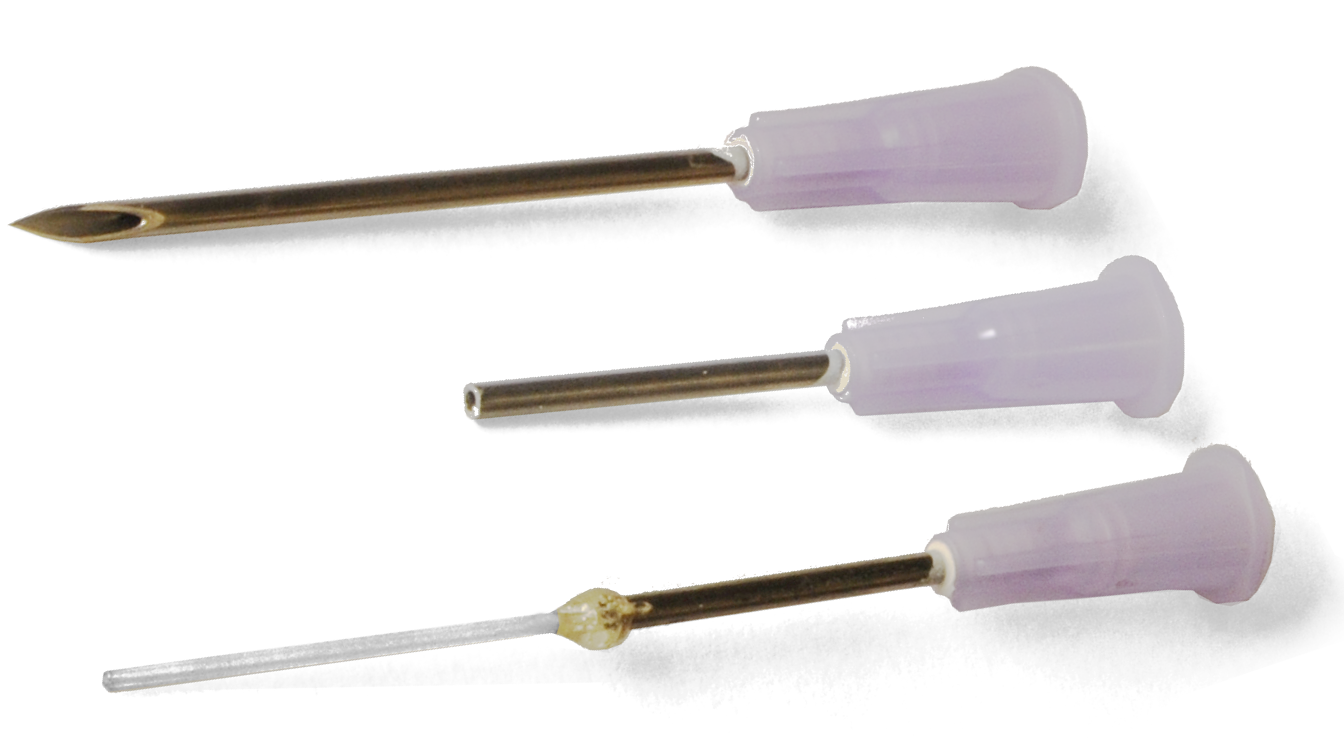
\includegraphics[width=0.4\textwidth]{img/setup/needles.png}
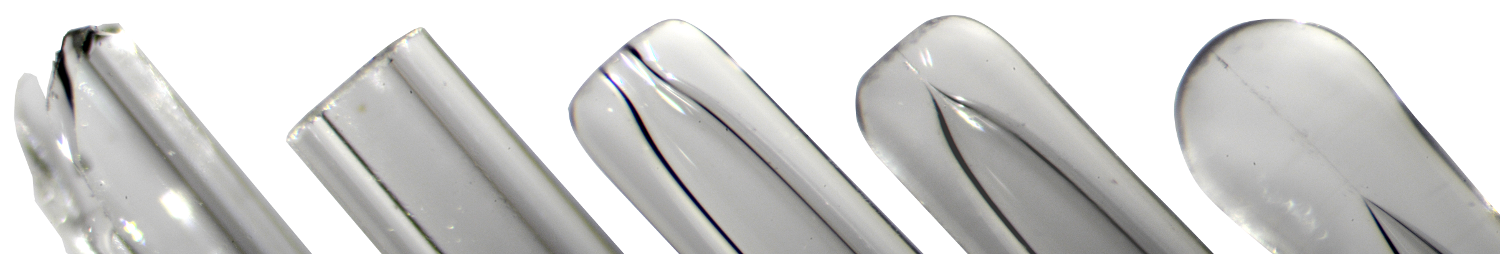
\includegraphics[width=0.35\textwidth]{img/setup/needletips.png}
\caption{Above: assembly of nozzle from
low-gauge hypodermic syringe (Luer fitting) and capillary. Below: nozzle tip
fabrication, capillary from left to right: broken, sanded, heated in a flame (I.D.
$200\,\mu$m), heated for longer (I.D. $25\,\mu$m, could be sanded down by about
$200\,\mu$m), overheated (I.D. $0\,\mu$m). \label{fig:needles}}
\end{wrapfigure}
If possible, forgo multi-platter drives, as they are more cumbersome to disassemble and have
bulky, complex actuator assemblies. The device shown in \figref{fig:harddrive-photo}
is based on a single-platter drive.

\paragraph{Dismantle and cut.} After removing the hard drive cover, remove
the magnet holder, arm axis, arm, ribbon wires, circuit boards, and platters
such that only the base plate remains. Now the corner of the base plate holding
the actuator arm assembly can be cut out to yield the result shown in
\figref{fig:designschematic}. A band saw, jigsaw or powered hacksaw will be
very useful, although not necessary. The goal is to allow the tip of the arm to
protrude over the edge.

\paragraph{Expose coil leads.} Next, remove the read/write head and all
wiring leading to it, along with any connected I/O and servo circuitry. Be
careful, however, not to tear off the two strands powering the voice coil. If
they are integrated in a ribbon you wish to remove, ensure that exposed
terminals remain onto which you can solder new leads.
\begin{figure}
\centering
        \begin{subfigure}[b]{0.45\textwidth}
            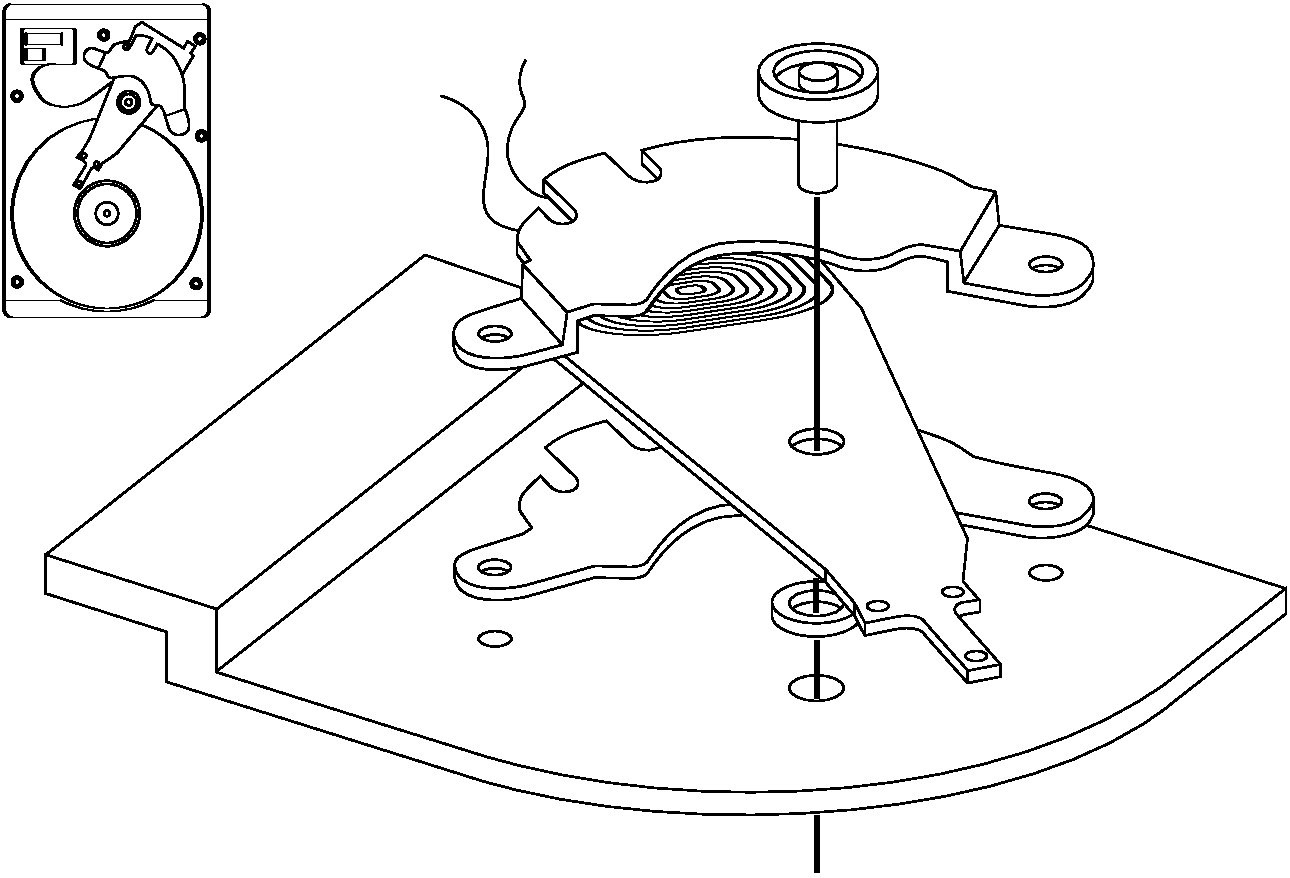
\includegraphics[width=\textwidth]{img/setup/dropletgenerator_exploded.pdf}
            \caption{\label{fig:harddrive-photo}}
        \end{subfigure}~\begin{subfigure}[b]{0.45\textwidth}
            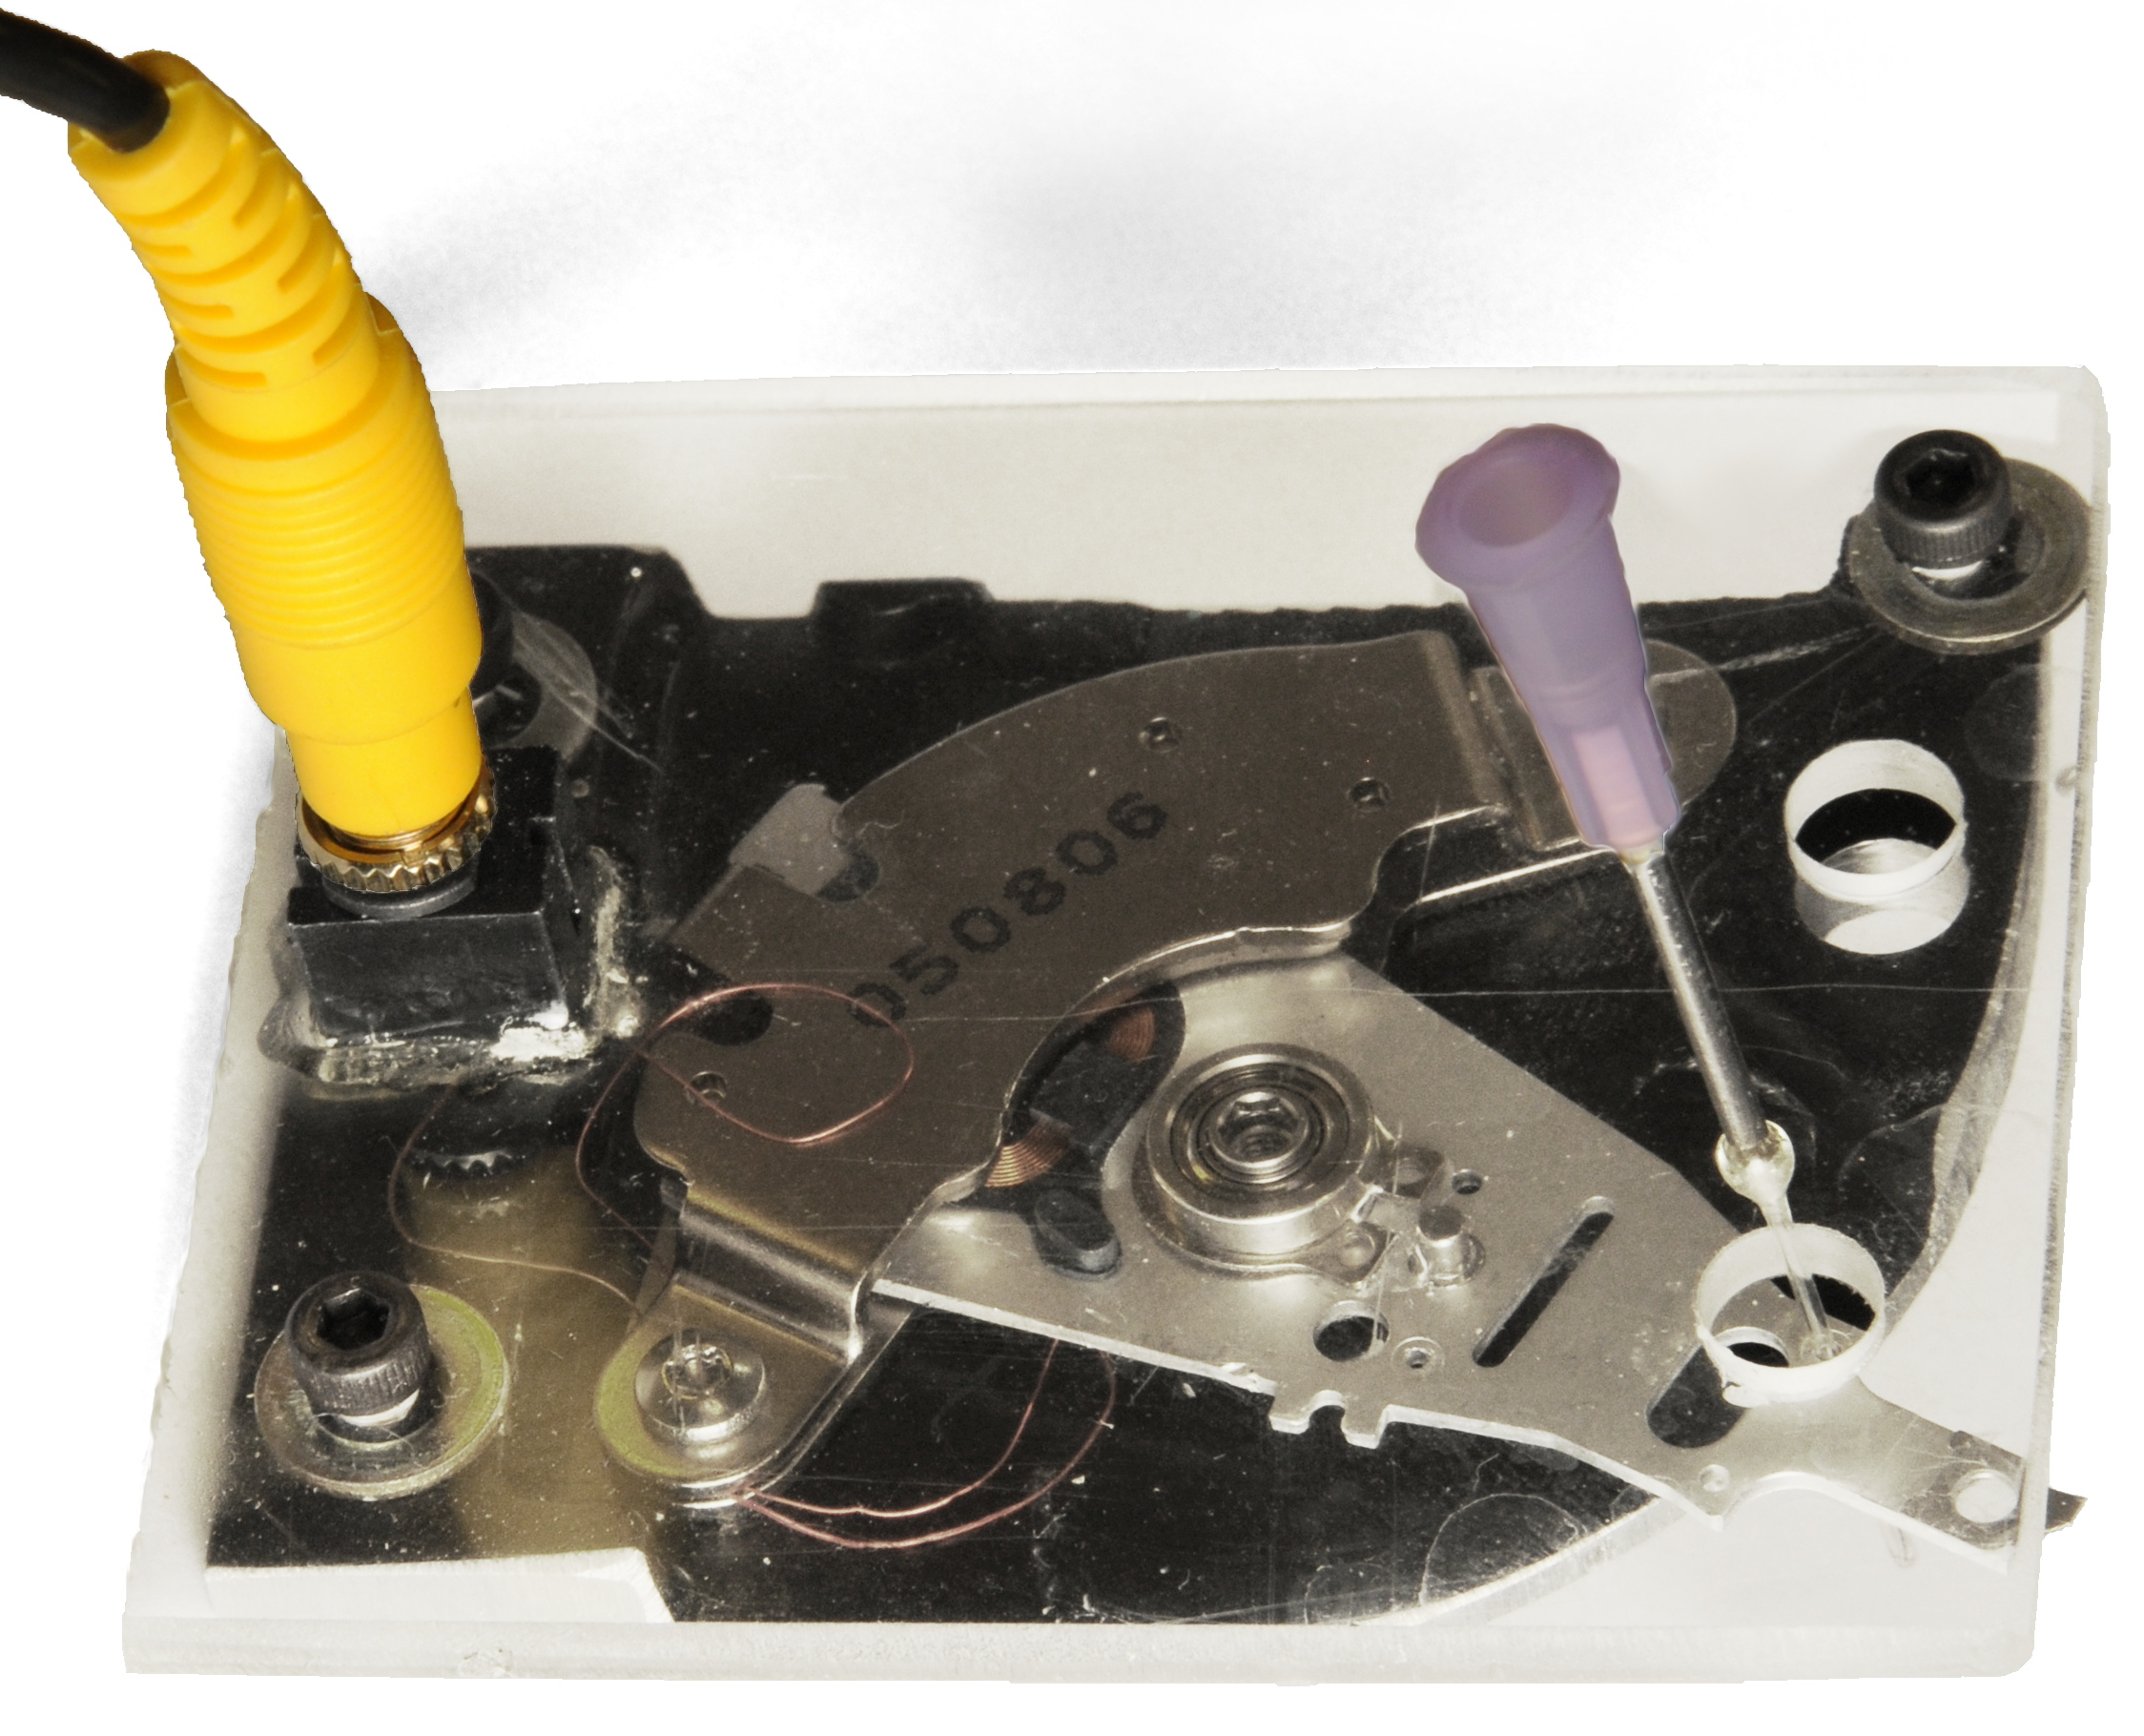
\includegraphics[width=\textwidth]{img/setup/designpicture.jpg}
            \caption{\label{fig:designschematic}}
        \end{subfigure}
        \caption{(a) top view of a hard drive and exploded view of the cut-out base
        plate, actuator arm, axis, and magnet assembly; (b) assembled droplet
    generator with cover plate and nozzle inserted through actuator arm.}
\end{figure}
\paragraph{Add protective cover.} We recommend bolting on a cover plate, such
as a small sheet of acrylic or polycarbonate, to protect the protruding arm from
accidental bending. Drill a hole through the cover to allow the nozzle to be
threaded through the arm. A severable
connection from coil to function generator is preferable to a direct wire, if
only because the voice coil leads are delicate and easily torn off. To this end, we epoxied
an audio jack into the cover and soldered the voice coil leads to it from the
bottom. 

\subsubsection{Operation}
To use the droplet generator, simply insert a nozzle through a small hole at the
tip of the actuator arm---typically at least one hole will already be present, but you may wish to drill
more---and connect the voice coil leads to the output terminal of a function
generator set to an initial peak-to-peak voltage of $1\,$V and a sinusoid frequency of
about $50\,$Hz, which should cause weak but perceptible oscillations.


We used existing nozzles manufactured by hand from hypodermic needle stubs and
heated glass capillaries (\figref{fig:needles}). We make no claim that this is
the best approach to take, but we note that the interchangeability of nozzles
with Luer fittings has proved very convenient in our application. How the nozzle
can be held in place falls beyond the scope of this article; while we used an
existing setup made from machined aluminum, a small lab stand and clamp should
suffice to hold the male Luer fitting connecting the feed tube to the nozzle.

The nozzle must be supplied by an accurately calibrated syringe pump. It is
convenient to integrate a large liquid reservoir (or tap water hose) via a
T-valve between the between pump and nozzle to permit quick topping up of the
syringe. In such a setup ensure that the reservoir valve is shut closed before operation,
since pressure fluctuations at the nozzle are the most common culprit for
unstable jet breakup conditions.

As with other vibrating orifice droplet generators, it is crucial that stable
conditions are established before any experiments can begin. First, confirm that
the liquid is ejected in a single jet. Multiple jets can be due to a clogged
orifice (a mixture of distilled water and CLR®, drawn back through a
syringe, is an excellent remedy). Satellite droplets can also form secondary
jets, in which case the oscillation frequency must be adjusted or the amplitude
reduced. Satellite formation is easily detected by using a gentle air flow to
deflect the jet---if the droplets are truly monodisperse, they will all deflect
at the same angle.\cite{Strom69}


\section{Determining the produced droplet size}
With droplet generators based on Rayleigh breakup, such as the HDG, this is easy
to do; just take the flow rate and divide by the number of droplets produced per
second (which, under stable conditions, equals the vibration frequency as each
instability turns into one droplet). If we assume perfect sphericity, we can
convert this droplet volume into a diameter. After cancelling terms, the
expression for $D_d$ becomes
\begin{equation}
    D_{d} = \sqrt[3]{\frac{6Q}{\pi f}}\label{eq:dropdia-continuous}
\end{equation}

The reliablity of the underlying assumption has been verified photographically
for several different nozzle orifice diameters and frequencies, some of which
are given as part of the ILIDS calibration.

\subsection{Photographing droplets}
With drop-on-demand approaches, the diameter of the produced droplet is more
difficult to predict, particularly since not the whole squeezing volume may
result in ejected liquid (e.g. with the Chandra generator, it's just a small
droplet). So to find out how big these droplets are (or just to verify the accuracy of
Eq.~\eqref{eq:dropdia-continuous}), we must resort to photographic means.

While there are different methods of photographing droplets, just taking
pictures in front of a strobe light has worked well.

We used a scale placed next to the droplet stream, and then used a conversion
between pixels to find the size. Of course, this method suffers from barrel
distortion that inevitably happens, especially with a zoom lens. 
% TODO: measure the barrel distortion.
\begin{wrapfigure}[19]{L}{0.4\textwidth}
\centering
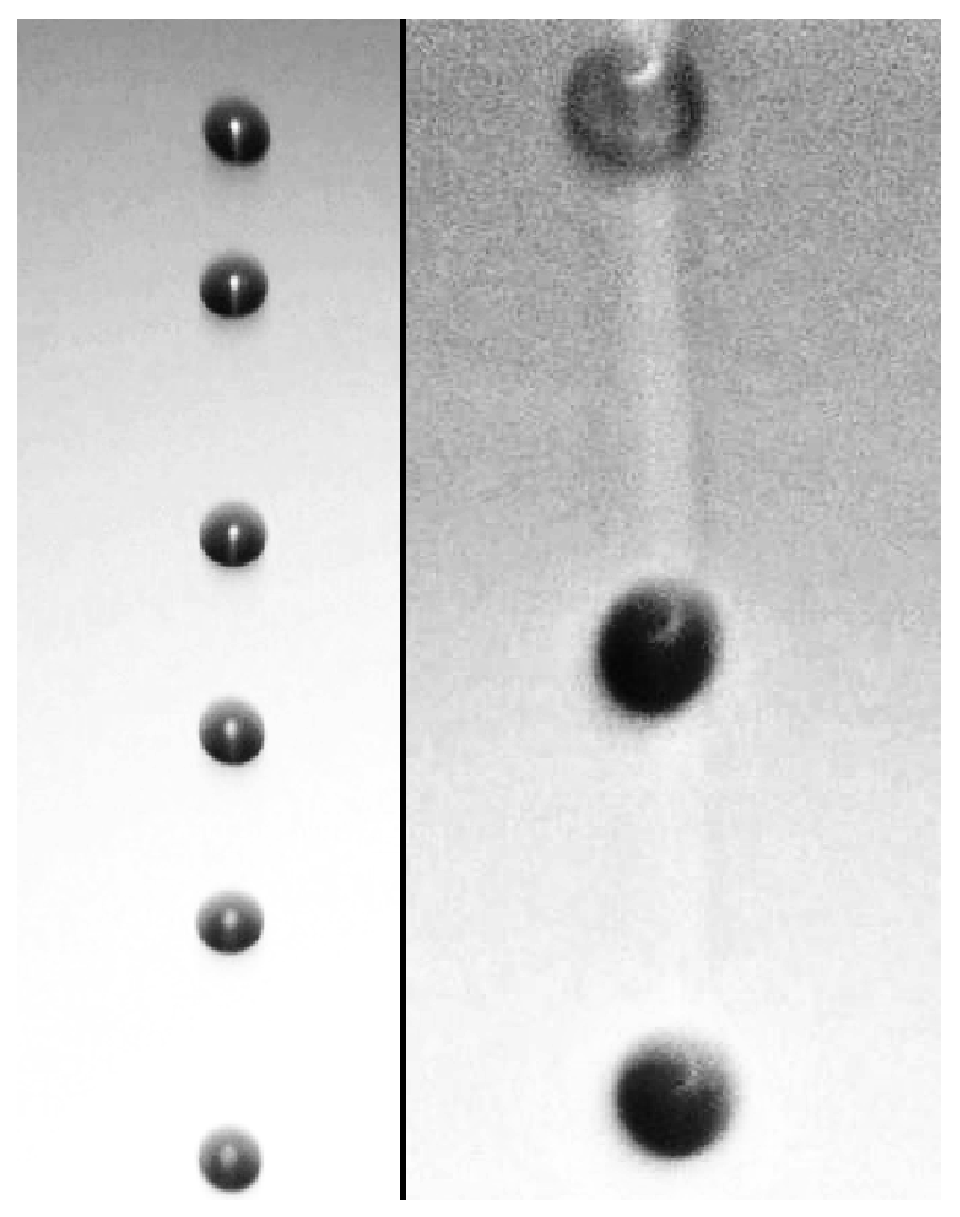
\includegraphics[width=0.35\textwidth]{papers/hdg_images/photo.eps}
\caption{Photographs of different droplet sizes ($220\,\mu$m and $386\,\mu$m,
    $f=1.990\,$kHz and $1.065\,$kHz respectively) produced with the droplet
generator shown in \figref{fig:hdg-photo}. Scales have been cropped out.
\label{fig:hdg-dropphoto}}
\end{wrapfigure}
Figure X shows a typical droplet stream photo (at different sizes).

\subsection{Droplet collisions}
\label{sec:droplet-collisions}
No droplet generation mechanism is perfect. Small fluctuations in flow rate,
unwanted harmonic vibrations and air turbulence can cause disturbances in the
stream of evenly spaced droplets -- the smaller the droplets, the more often
this happens. Occasionally, this will lead to the collision
of two droplets some distance away from the orifice.

When two drops of diameter $D_d$ collide, the diameter of the new droplet equals
\begin{equation}
    D_{d+d} = 2\sqrt[3]{2\left(\frac{D_d}{2}\right)^3} = \sqrt[3]{2} D_d \approx
    1.26 D_d.
\end{equation}

Indeed, secondary peaks will often appear in diameter histograms at precisely 126\% of
the peak diameter. As long as the underlying phenomenon is understood and kept
under control, these secondary peaks should be no cause for concern during the
calibration. Typically, photographs will confirm that a few droplets go astray
and collide with others. Since the ``real'' diameter peaks are easily discerned,
the secondary peaks can simply be ignored.

\chapter[ILIDS]{ILIDS}
Interferometric Laser Imaging for Droplet Sizing (ILIDS), also known as
Interferometric Particle Imaging (IPI) and MSI (Mie Scattering Imaging) is an
optical droplet sizing method in which a spray is illuminated by a sheet of
laser light and the scattered light is imaged laterally. The laser light is both
reflected and refracted by the droplets, such that each droplet produces a pair
of apparent ``glare points''. When seen through a lens away from the focal
plane, each pair of glare points---being sources of coherent monochromatic
light---appears as an interference pattern which, after falling through a
circular aperture, casts an image that is a circular disk of fringes.  The
spatial frequency of the fringes is (to a very close approximation) linearly
related to the particle size. The phenomenon was first described by
\citet{Konig86} and later in greater detail by \citet{Glover95}. Turnkey ILIDS
setups for spray characteriziation are now widely available, comprising
typically a pulsed Nd:YAG-laser, one or two CCD cameras, a timing circuit, and a
piece of image processing software.

\begin{figure}
\centering
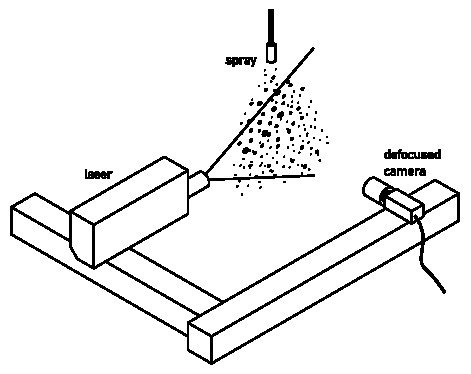
\includegraphics[width=0.7\textwidth]{img/setup/ipi_setup_simple.pdf}
\caption{Perpendicular ($\phi=90^\circ$), single-camera ILIDS setup
\label{fig:ipi-setup-simple}}
\end{figure}
\section{Operating principle}
The number of fringes $N_\text{fr}$ appearing in the image has a simple linear relationship to
the droplet diametre $D_d$:
\nomenclature{$N_\text{fr}$}{Number of fringes}
\nomenclature{$\kappa$}{Scalar value relating the fringe count $N_\text{fr}$ to
the physical diameter of the particle $D_d$}
\nomenclature{$D_d$}{Physical diameter of the particle (here: droplet)}
\begin{equation}
    N_\text{fr} = \kappa D_d,
\end{equation}
where $\kappa$ is a constant derived from the optical configuration:
\begin{equation}
    \kappa = \frac{\arcsin\left(\frac{D_a}{2z}\right)}{\lambda}
    \left(\cos\frac{\phi}{2} - \frac{m \sin\frac{\phi}{2}}{\sqrt{m^2 + 1 -
    2m\cos \frac{\phi}{2}}}\right).
    \label{kappa}
\end{equation}

In the above expression $D_a$ is the aperture diametre, $z$ is the distance of
the lens to the laser sheet, $\phi$ is the off-axis angle (90 degrees in most
setups, including ours), and $m$ is the relative refractive index of the
droplets (1.333 for water in air).

As a consequence of geometrical optics, the distance $s_x$ (in pixels) between two
adjacent fringes has a linear relationship with the defocussing distance $\Delta
z$, where $M$ is the magnification, $d_{p,x}$ is the physical size of a
camera sensor pixel, and $\Delta \theta$ is the angle subtended by two adjacent
fringes entering the lens \cite{Pan06}:
\nomenclature{$\Delta \theta$}{Angular spacing between two adjacent fringes}
\nomenclature{$\Delta z$}{Distance along the $z$-axis between the focal plane of
the lens and the light sheet}
\nomenclature{$M$}{Magnification}
\nomenclature{$s_x$}{Distance, in pixels, between two adjacent fringes}
\nomenclature{$d_{p,x}; d_{p,y}$}{Physical dimensions of a pixel on the camera's
CCD sensor}
\begin{equation}
  s_x = \frac{\Delta \theta \Delta z}{M d_{p,x}} 
  \label{fringedistance-pixels}
\end{equation}
Of course, equation \eqref{fringedistance-pixels} is only meaningful where $\Delta z \gg
0$. When the image is brought into focus ($z\approx 0$), fringes will give way to a sharp
image of the glare points.\footnote{To be exact, diffraction will
cause every point to be imaged as an Airy disk, but we shall neglect
this effect here.} Of course, if the pixel density is too low to resolve
both glare points, a single bright spot will appear. 

\subsection{Influence of the scattering angle $\phi$}
The scattering angle $\phi$, illustrated in \figref{fig:droplet-rays}, determines the
relative contribution of different scattering orders of light to the imaged
fringe pattern. Both geometric optics \cite{Vandehulst12} and Mie theory provide
methods to compute the total scattered intensity for a given $\phi$ and $m$;
some examples can be found in \citet{Kawaguchi02} and \citet{Mounaim99}. The
geometric analysis approach is not valid beyond $\phi > 70^\circ$, as the
first-order scattered beam ($p=1$) is not visible from this angle
\cite{Glover95}.

\begin{wrapfigure}[14]{R}{0.5\textwidth}
\centering
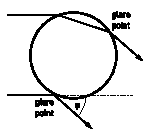
\includegraphics[width=0.4\textwidth]{img/setup/droplet_rays.pdf}
\caption{Reflected and first-order-refracted light rays, producing two glare
points when viewed from an angle $\phi$. \label{fig:droplet-rays}}
\end{wrapfigure}

While authors have identified several forward angles as optimal for their
applications, e.g. $\phi = 45^\circ$ \cite{Glover95} or $\phi = 66^\circ$
\cite{Mounaim99}, such configurations inevitably result in a variation in $z$,
and therefore defocusing, across the image unless the
camera itself is angled with respect to the lens to correct for this aberration
(the so-called \emph{Scheimpflug condition}). Since the latter approach requires
specialized optical equipment, $\phi = 90^\circ$ is used in many setups,
including the one in this paper.

\subsection{Optical limits on fringe detection}
\label{sec:ipi-fringelimits}
Optics impose theoretical and practical size limits on the droplets to be
measured. We will outline them in the following paragraphs; the reader is
referred to \citet{Damaschke02} for a more detailed analysis.

\paragraph{Nyquist criterion for the fringe density.}
The Nyquist criterion requires that for the camera to be able to resolve a pair
of neighbouring fringes, their images must be at least two pixels apart. This
can easily be achieved by a sufficient defocusing the lens, which widens the
fringe image, increasing the number of pixels covered by each fringe. The lens
mechanics permitting, any arbitrarily large droplet can thus be measured after a
quick adjustment. In theory, this correction is effective until the defocused
droplet image is too large for the CCD sensor, and fringes are cut off. In
practice, overlap and noise (see below) will cause significant problems long
before the image can be defocussed beyond the sensor edges.

\paragraph{Signal-to-noise ratio.}
Image noise is a significant source of trouble in ILIDS analysis. Indeed, many
droplet images must be discarded as data sources because they are too weak
compared to the noise.
Small droplets suffer from this more than larger ones because they scatter less
light,\footnote{The scattered intensity grows with the cross-section of the
droplet} but the problem also occurs with deeply out-of-focus images of very large
droplets, as dilated droplet images spread the same amount of light over a
greater area on the camera sensor. As a result, they are darker on average than
less defocused images. 

\paragraph{Minimum droplet size.}
\citet{Damaschke02} argue that the smallest measurable droplet is one that
produces exactly one fringe falling through the aperture. We may speculate that, at least
in theory, the fringe frequency should be measurable even if only a partial
fringe is shown. This would require its image to be sufficiently zero-padded
before the Fourier transform is applied to it. In practice, however, the
intensity of scattered light typically drops below an acceptable level well before
the fringes become too large, and noise (see above) will become the overwhelming
problem.

\paragraph{Deviation from actual Mie scattering for small droplet sizes.}
ILIDS users should also be aware that the assumptions of geometric optics
that underlie \eqref{kappa} do not hold for small droplets. \citet{Mounaim99}
found that for isooctane droplets ($m=1.39$) below $10\,\mu$m, geometric optics
yield a fringe spacing value about 14\% higher than that predicted by exact Mie
scattering simulations at $\lambda=532\,$nm. While the deviation quickly
vanishes for larger droplets, it is nevertheless noteworthy in the context of
potential error sources.

\paragraph{Overlapping droplet images.}
The ability to image a whole 2D field of droplets all at once is ILIDS' strongest
selling point, yet also its curse. When droplets are spaced too closely and the
lens is sufficiently defocused, the defocused disk images overlap and it becomes
difficult to determine the fringe counts corresponding to individual droplets.
\citet{Damaschke02} provide a statistical estimate on the fraction of
overlapping disks (overlap coefficient). 


\section{Types of ILIDS setups}
\label{sec:ipi-setup}
\subsection{Standard ILIDS}
The most simple ILIDS configuration, as shown in \figref{fig:ipi-setup-simple},
consists of a single digital camera with a defocused objective lens, placed at a right
angle to the laser sheet. The lens aperture is (approximately) circular and
typically completely open to permit as much light as possible to fall on the
sensor area.

Both camera and laser are connected to a computer via a timing circuit, and both
can be triggered simultaneously by software installed on the computer.
Commercial ILIDS vendors provide the timing circuitry and the software, which
typically integrates a collection of image processing algorithms that can be
used to analyze the captured images immediately.

The core problem with all ILIDS setups is the determination of $z$ and $d_a$ in
\eqref{kappa}.  We will discuss calibration of ILIDS systems in greater detail in
\secref{} calibration.

Images taken in this configuration are very susceptible to excessive
disk overlap.


Therefore, measures have been developed to sidestep overlap
almost entirely or to deal with it during the image processing stage. These
modifications will be described in the next sections.

\subsection{ILIDS with optical compression}
This problem is never more apparent than in efforts to calibrate
the system using a vibrating orifice droplet generator, as the droplets produced
thereby are spaced very closely and produce heavily overlapping defocussed
images. Fortunately, there exists a simple and reliable technique to deal with
this problem: a slit aperture, installed directly in front of the lens, masks
the defocussed droplet images such that only a thin strip across their center
passes through the lens. The effect is shown in \figref{fig:globalsizing}. 

Arguably the most popular way to reduce the amount of overlap is the use of
optical compression techniques, whether by means of a slit aperture \cite{Pan06}
or a cylindrical lens \cite{Kawaguchi02, Maeda02}. However, some techniques
(e.g. Global Phase-Doppler \cite{Damaschke01} and intensity-analyzing
methods \cite{Querel10}) or use cases (e.g. very low signal-to-noise ratios)
require the full disk image to be available. In these cases, the standard
approach is to identify the location and outline of each disk image, such that
the fringe analysis can either be limited to non-overlapping regions or be
otherwise modified to take overlapping fringes into account.

Naturally, equations \eqref{kappa} and \eqref{fringedistance-pixels} still hold.
\begin{figure}[h!]
    \centering
    \begin{subfigure}[b]{0.4\textwidth}
        \centering
        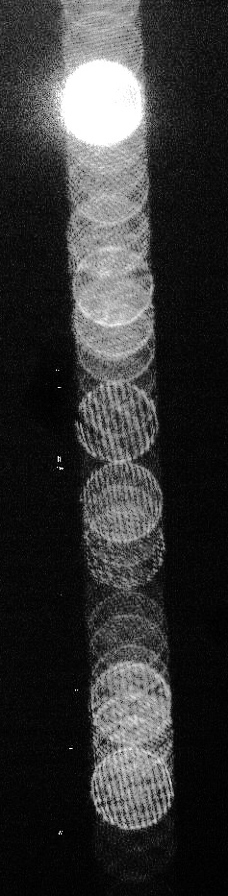
\includegraphics[height=0.6\textheight]{img/dots_cropped.jpg}
        \caption{}
    \end{subfigure}
    \begin{subfigure}[b]{0.4\textwidth}
        \centering
        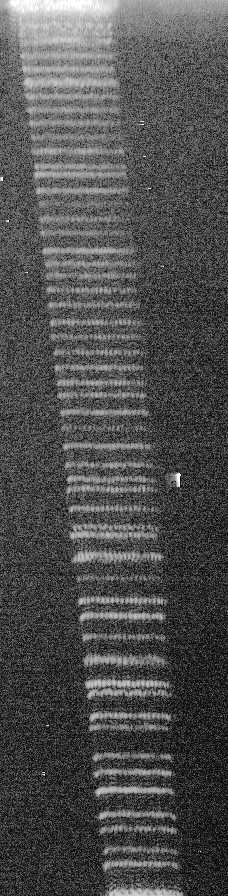
\includegraphics[height=0.6\textheight]{img/slitted.jpg}
        \caption{}
    \end{subfigure}
    \caption{Before (a) and after (b) installing the slit aperture. The aperture
    stop pares off the top and bottom halves of the defocussed circles, leaving
only a narrow center string in the middle.}
    \label{fig:globalsizing}
\end{figure}
Also mention that this can be used in conjecture with an additional, focused
camera, to capture things like speed (PIV), evaporation (PLIF), etc. Why we
don't need it.

Extracting the fringe counts from such an image is straightforward. First, we
correlate the image with that of a single, solid bright rectangle which shares
the approximate dimensions of a typical strip in the image. This operation
yields intensity
peaks centered over our regions of interest. We remove closely adjacent peaks,
as they may represent questionable or overlapping strips. Compared to the sheer
number of correctly identified strips, the number of legitimate data points lost
this way is negligible. \figref{fig:globalsizing-identifystrips} shows the
result of such an attempt at identifying the strips.

\begin{figure}[h]
    \centering
    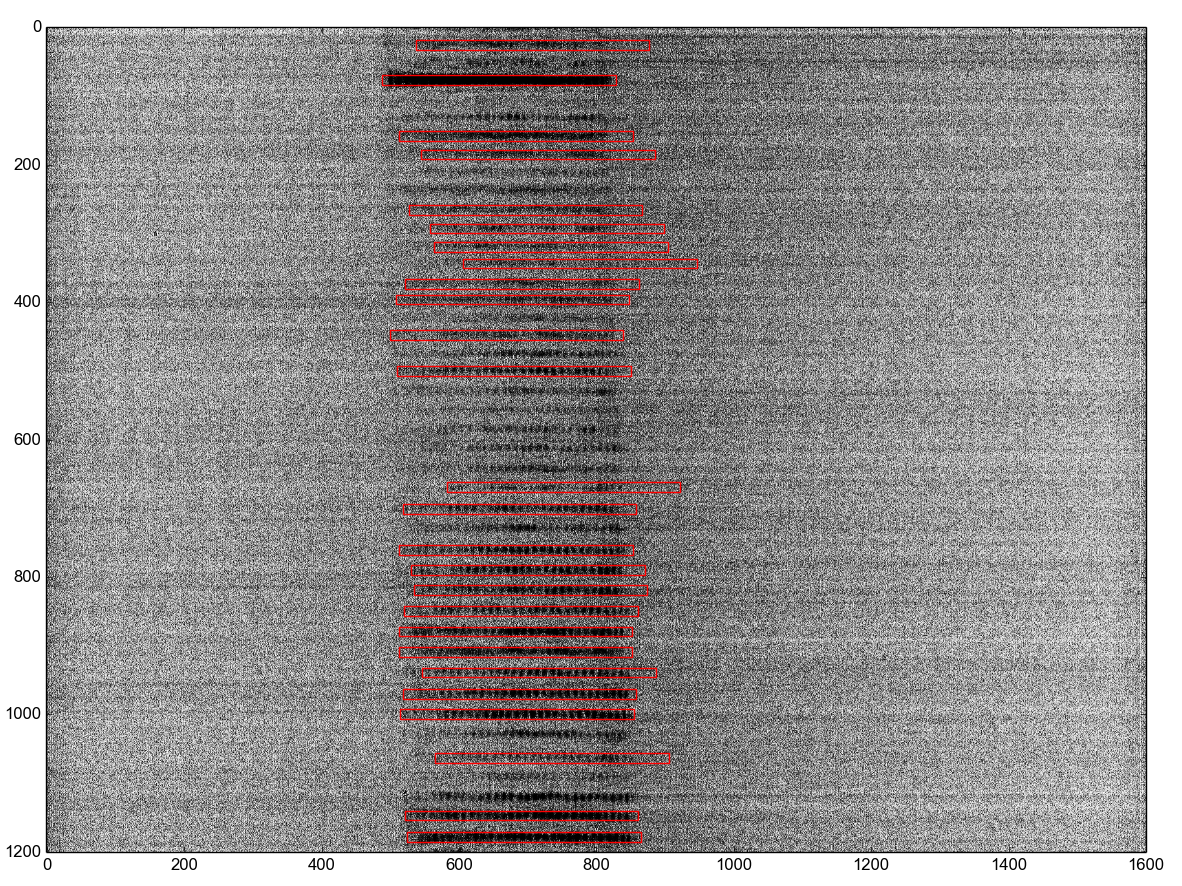
\includegraphics[height=0.38\textheight]{img/globalsizing-identifystrips.png}
    \caption{The image is correlated with that of a solid bright rectangle, which
        results in peaks that approximately coincide with the centers of the
        strips. Here, the original photo is shown with rectangles drawn centered
    at said peaks.}
    \label{fig:globalsizing-identifystrips}
\end{figure}

To find the number of fringes within the strip, we cannot rely on counting the
number of dark/bright variations directly, as some of them may be lost in the
noise. The spatial frequency of the peaks, however, taken together with the
known and constant horizontal width of the strips, will produce a reliable
fringe count. In the next step, our algorithm therefore applies the Fourier
transform to each region of interest. To improve the accuracy of the method,
three steps are performed before the Fourier transform is taken:
\begin{enumerate}
    \item a weak ($3 \times 3$) Gaussian blur is applied to the region
        (optional);
    \item a Hanning window is applied to the region -- both horizontally and
        vertically. This reduces the ``sinc ringing'' effect encountered when
        taking the Fourier transform of finite signals;
    \item the region is padded with zeros in all directions to yield a larger
        input to the Fourier transform. In our application, the windowed and padded strip
        images had dimensions of $1024 \times 1024$ pixels. Zero-padding
        increases the granularity of the frequency spectrum, which can help with
        the correct identification of the peak frequency.
\end{enumerate}

\figref{fig:globalsizing-dropletpeak} shows the windowed appearance of
one such region of interest (although it does not show the padded input to the
Fourier transform due to space constraints). The Fourier transform yields a
frequency power spectrum in two dimensions, although we are primarily interested
in the frequency peak in the horizontal direction (i.e. along $y=0$). In order
to minimize the misidentification of dominant frequencies,
\begin{enumerate}
    \item we clip the spectrum to a band of reasonable frequencies. This is
        necessary because a) $1/f$-noise causes very low frequencies to dominate
        in power, although they are of no interest to us, and b) graininess in
        the original photo can sometimes result in meritless high-frequency
        peaks;
    \item we apply a Gaussian blur to the 2D spectrum to remove outliers in the
        spectrum;
    \item we discard all regions in which the peak frequency's power does not
        exceed a certain value;
    \item we discard all regions in which the \textit{prominence} of the peak
        freqency's power (i.e. its proportion to the mean power) does not exceed
        a certain value (this step is optional).
\end{enumerate}
The bottom two elements in \figref{fig:globalsizing-dropletpeak} illustrate
the effect of these steps.

\begin{figure}[h]
    \centering
    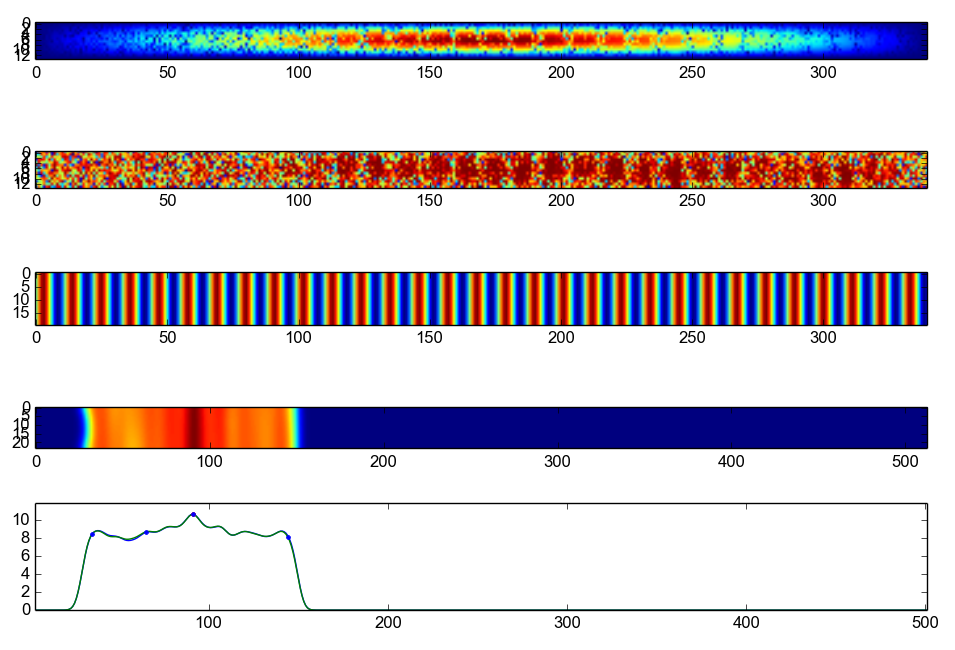
\includegraphics[height=0.38\textheight]{img/globalsizing-dropletpeak.png}
    \caption{From top to bottom: windowed region of interest; original
    (unwindowed) region of interest; sine wave representing the identified peak
frequency; clipped and lowpass-filtered 2D frequency spectrum showing a distinct
peak at about 90 oscillations across the image width of 1024 pixels; 1D plot of
the frequency spectrum, with peak identified at $f=91.0$.}
    \label{fig:globalsizing-dropletpeak}
\end{figure}

\begin{wrapfigure}[12]{R}{0.4\textwidth}
    \centering
    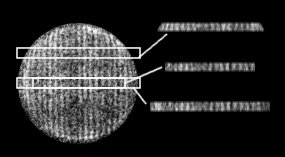
\includegraphics[width=0.35\textwidth]{img/dropletslitcropping2.jpg}
    \caption{Only a slit aperture centered on the lens and extending across the
    entire lens entrance will preserve all fringes \label{fig:droplet-slitcropping}}
\end{wrapfigure}
Finally, the peak frequency $f_\text{peak}$ is converted into a fringe count by re-scaling it
from the padded size $D_\text{padded}\, (= 1024$ pixels) to the width of the strip (which, in the
context of IPI measurements, should equal the diameter $D_\text{i}$ of the defocussed droplet
image):
\nomenclature{$f_\text{peak}$}{Peak frequency}
\nomenclature{$D_\text{i}$}{Diameter (in pixels) of the defocussed image}
\nomenclature{$D_\text{padded}$}{Width (in pixels) of the padded input to the
Fourier transform}
\begin{equation}
    N_\text{fr} = f_\text{peak} \frac{D_\text{i}}{D_\text{padded}}
    \label{fringes-from-diameter}
\end{equation}

While the above algorithm will generally give a good estimate of the fringe
count for a given defocussed droplet image, it cannot know whether the entire
center portion of the image has indeed passed the slit aperture. It is
conceivable, after all, that the slit aperture was not perfectly centered on the
lens entrance, or that the slit aperture was shorter than the diameter of the
lens entrance. \figref{fig:droplet-slitcropping} illustrates how the slit
aperture can cause the defocussed image to appear smaller than it is. The
reduced value for $D_\text{i}$, manually entered in equation
\eqref{fringes-from-diameter}, will result
in droplets being reported as smaller than they are in reality.

As noted above, ILIDS with optical compression can be used with an additional,
focused camera behind a beam splitter, as shown in
\figref{fig:ipi-setup-double}.\footnote{Alternatively, the two cameras may image
    the spray from different angles, e.g. as demonstrated by \citet{Glover95},
    although this complicates the setup as the Scheimpflug condition must be
fulfilled.} The latter may provide e.g. PIV images for a
velocity analysis or LIF images for evaporation studies. This was demonstrated
by \citet{Hardalupas10} and \citet{Hardalupas10a}. However, such setups suffer
from \emph{center discrepancies}. \secref{sec:point-set-registration} documents
how such center discrepancies can be dealt with.

\begin{figure}
\centering
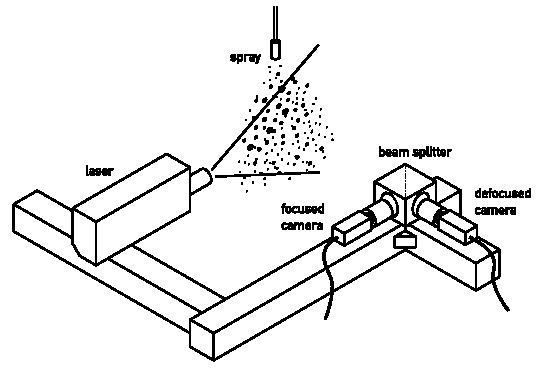
\includegraphics[width=0.75\textwidth]{img/setup/ipi_setup_double.pdf}
\caption{Perpendicular ($\phi=90^\circ$), double-camera ILIDS setup}
\label{fig:ipi-setup-double}
\end{figure}

\subsection{Additional focused image for disk detection}
As described above, running a simple frequency analysis on bright regions in an
ILIDS image is futile when two of the fringe disks overlap, as it is not clear
how many droplets are associated with the region and where their disks infringe.
While optical compression provides a very good solution to this problem, it is
not always applicable: some techniques (e.g. Global
Phase-Doppler \cite{Damaschke01} and intensity-analyzing methods \cite{Querel10})
or use cases (e.g. very low signal-to-noise ratios) require the full disk image
to be available. In these cases, the standard approach is to identify the
location and outline of each disk image, such that the fringe analysis can
either be limited to non-overlapping regions or be otherwise modified to take
overlapping fringes into account. Additionally, once disk centers are found, the
software can apply Hanning windows to the disks as well as ignore disk pairs
that are too close.\footnote{The latter is an effective control mechanism, but
    is liable to skew the representativeness of the sample because small,
dispersed satellites outside of the main flow are most likely to be validated.}

To identify the location of overlapping disks in the image, an additional camera
is introduced to capture a focused image of the spray simultaneously with the
defocused ILIDS camera. The setup is identical to that shown in
\figref{fig:ipi-setup-double}. The intensity peaks in the focused image are then taken
to be the droplet positions (i.e. disk centers) in the defocused image.

The problem with this, as with all multi-camera setups, are center
discrepancies. We show how to overcome that in
\secref{sec:keypoint-registration}.

\section{Calibrating the slit method}
What matters is the Numerical Aperture (NA), which is (the sine of half of) the
collection angle. When we have a simple lens, we can calculate this as
\begin{equation}
    \mathrm{NA} = \sin \frac{d_a}{2z}
\end{equation}

The Dantec manual suggests using the distance from light sheet to front of the
lens for $z$, and the ratio of min focal length and max f-number to find $d_a$.
This, however, does not result in an accurate value for the collection angle
with all lenses.

We are assuming, then, that the effective aperture (the entrance pupil) always
stays constant throughout the focussing range of the lens. This is not
necessarily the case, as there are lenses which change both the physical and the
virtual size of the aperture when focussing.

Here is where I make the claim that it is impossible to determine the actual
exact value for the numerical aperture of the lens. Similarly, it can be quite
difficult to determine the accurate distance from light sheet to lens aperture
(even though the latter measurement is more forgiving, since the distances are
far greater).

Taking into account the sources of errors explained in the sections above, it is
advisable to run a few calibration tests with droplets of different sizes before
employing the IPI technique for real spray measurements. Recall that, if we
ignore the Mie error (\secref{sec:mie-error}), the relationship between fringe count and droplet diameter
is linear with a constant of proportionality $\kappa$ (see equation
\eqref{kappa}). The aim of our calibration, then, is to determine the value of
$\kappa$ from experiment -- the premise being that we cannot be certain of the
values of $D_a$, $z$, and possibly not even $m$ and $\phi$ (although the latter
can usually be ascertained to a sufficient degree of accuracy).

\subsection{A sample calibration of the slit aperture method}
Using the droplet generator described in \secref{sec:droplet-generator} and
the IPI configuration described in \secref{sec:ipi-setup}, we produced and
measured monodisperse droplets of many different diameters. The droplet
diameters were determined both mathematically and photographically, as described
in \secref{sec:verify-droplet-diameters}. Out of over 30 sets of IPI
measurements we selected six sets that exhibited both strong uniformity and
high photographic quality:

\begin{table}[h!]
    \centering
    \begin{tabular}{lrrrrr}
    \toprule
    Set & Flow rate & Frequency & $D_d$, predicted  & $D_d$, from
photo & $\hat{N}_\text{fr}$ \\
    \midrule
    FA & 20.8  ml/h  & 5395 Hz  & 127 $\mu$m  & 126 $\mu$m &  9.71      \\
    FB & 39.7  ml/h  & 1990 Hz  & 220 $\mu$m  & 226 $\mu$m &  16.71     \\
    FC & 79.4  ml/h  & 1565 Hz  & 299 $\mu$m  & 291 $\mu$m &  22.92     \\
    FD & 94.3  ml/h  & 1067 Hz  & 361 $\mu$m  & 367 $\mu$m &  27.26     \\
    FE & 114.1 ml/h  & 1065 Hz  & 384 $\mu$m  & 384 $\mu$m &  29.89     \\
    FF & 175.2 ml/h  & 1038 Hz  & 447 $\mu$m  & 454 $\mu$m &  34.56     \\
    \bottomrule
\end{tabular}
\caption{Six sets of calibration data taken with the setup described in \secref{sec:ipi-setup}}
\label{tab:ipi-calibration-datasets}
\end{table}
\nomenclature{$\hat{N}_\text{fr}$}{Peak fringe count measured}
The values for $\hat{N}_\text{fr}$, the peak fringe count, are based on the
histograms (see \figref{fig:fringe-histograms}) showing the distribution of
fringe counts within each dataset. These fringe counts are of course found by
the algorithm described in \secref{sec:ipi-slitprocessing}.

It is worthwhile to point out some apparent idiosyncrasies in the histograms of
datasets FB and FC. Their peak fringe counts are 16.71 and 22.92, but there are
secondary peaks at about 21 and 29 fringes, respectively. The latter are
explained by the collision of droplets as discussed in
\secref{sec:droplet-collisions}, and are ignored for the purposes of
calibration.

\begin{sidewaysfigure}[p]
    \centering
    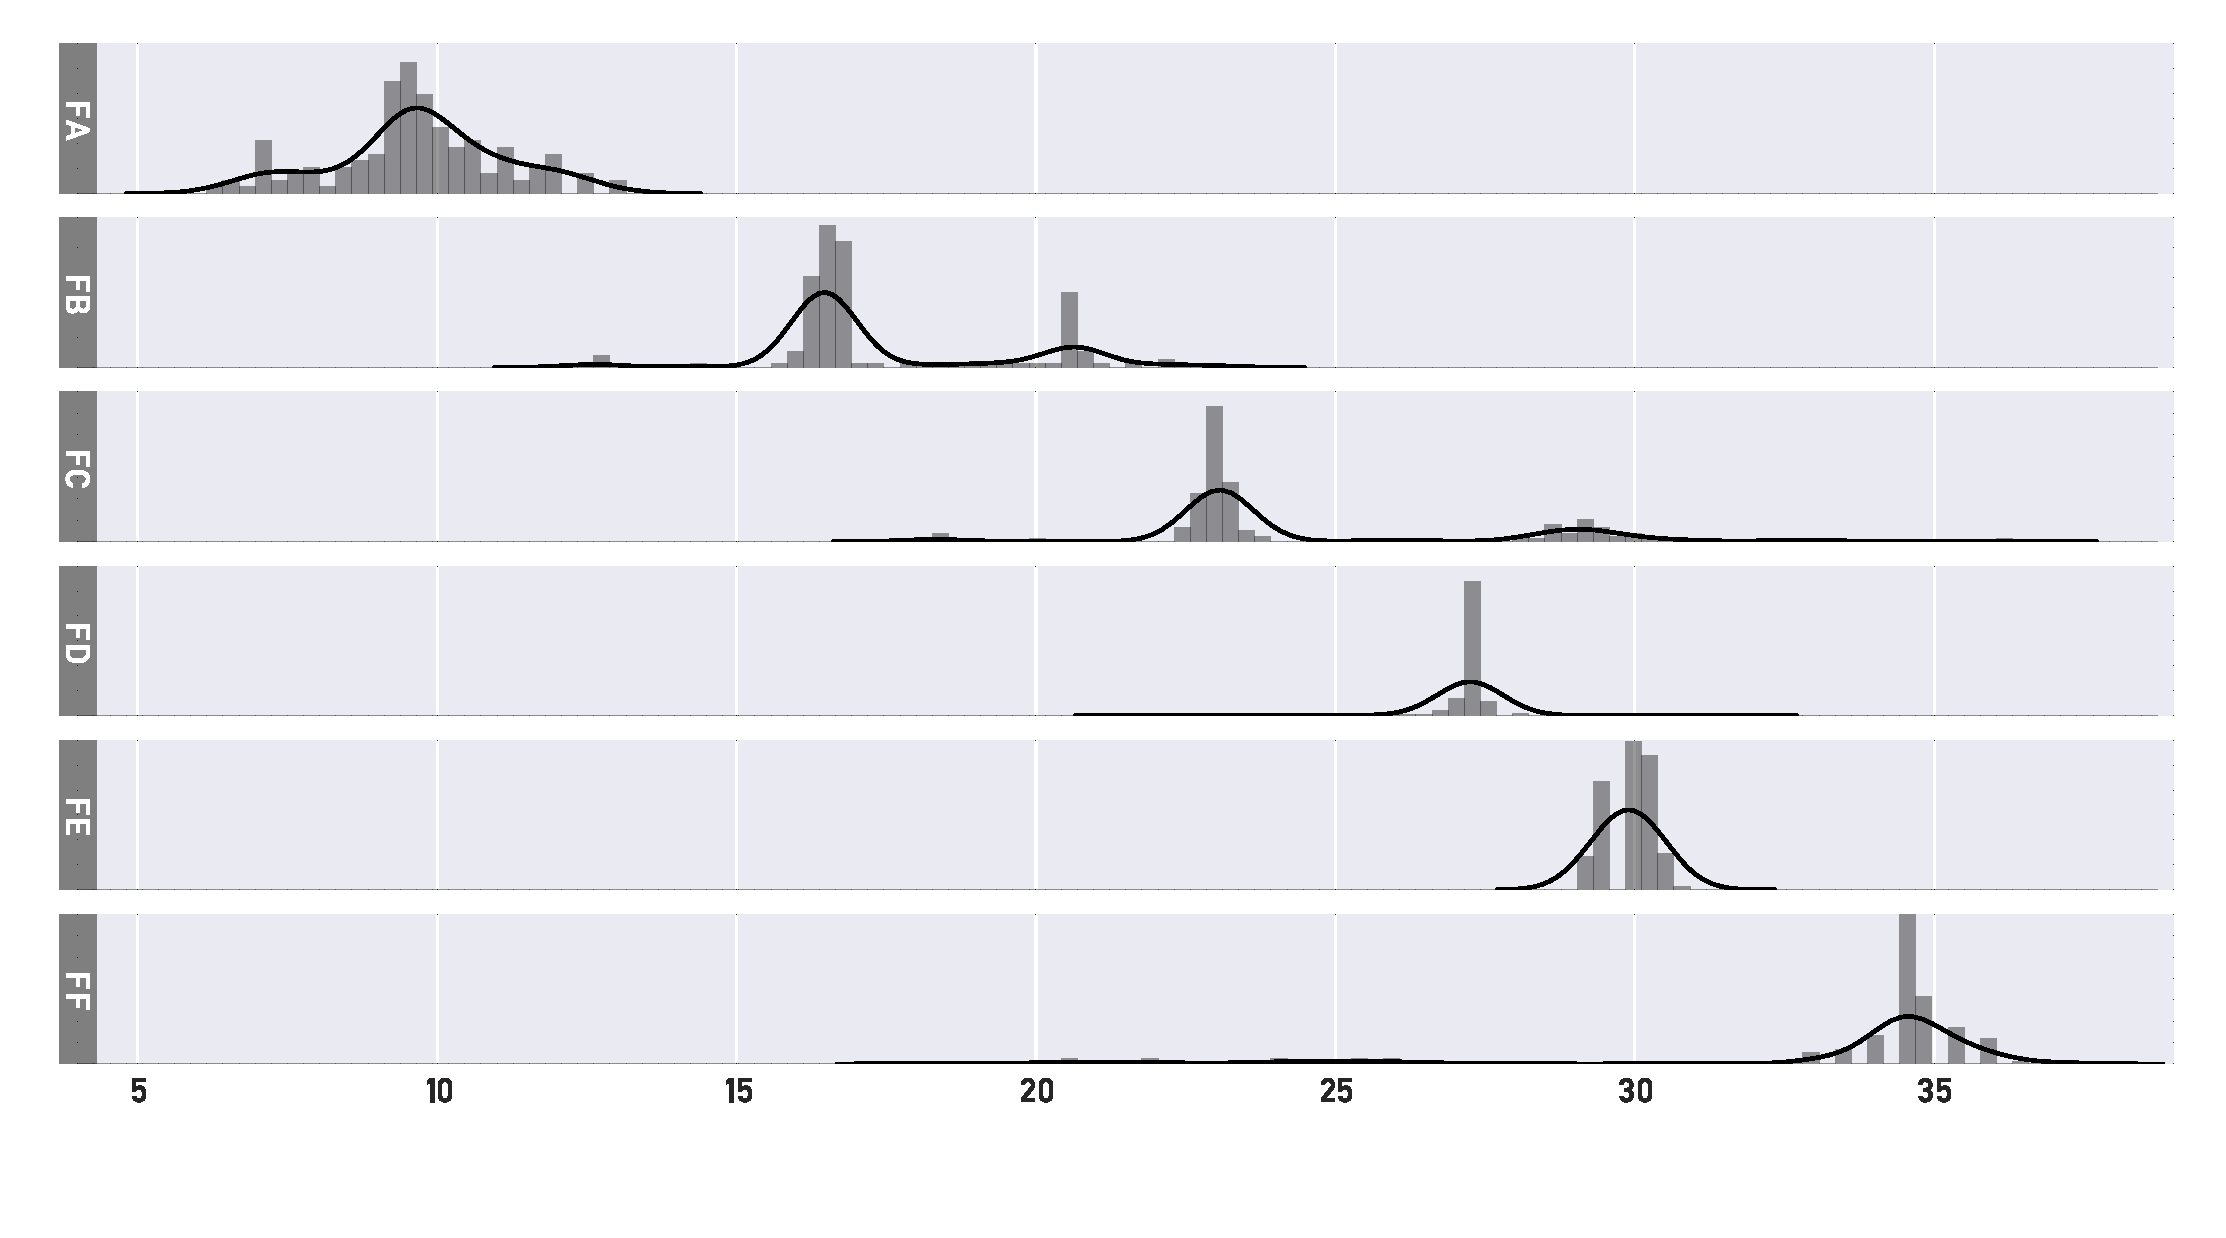
\includegraphics[width=\textwidth]{img/fringe_histogram.pdf}
    \caption{Normalized distributions of measured fringe counts $N_\text{fr}$
        for the six datasets listed in \tableref{tab:ipi-calibration-datasets}. Solid lines are
Gaussian kernel density estimates with $h=0.5$. }
    \label{fig:fringe-histograms}
\end{sidewaysfigure}

The close agreement of the droplet diameters found from photographs with those
predicted by \eqref{berglund} reassures us that we can use the predicted $D_d$
for further analysis.

At this point, we can least-squares-fit the linear relationship \eqref{kappa} to the primary
peaks $\hat{N}_\text{fr}$ and the known droplet diameters $D_d$ to find
$\hat{\kappa}$:

\begin{equation}
    \hat{\kappa} = \frac{\sum_i D_{d,i} \, \hat{N}_{\text{fr}, i}}{\sum_i
    D_{d,i}^2}
\end{equation}

Note that instead of the standard least squares regression we here use a
simplified formula to force the trend line through the origin. This choice
should not be made lightly, since it will usually cause the residuals to have a
non-zero mean. In this case, however, we believe it to be justified to require
that $D_d = 0$ for $N_\text{fr} = 0$.

Based on the values in \tableref{tab:ipi-calibration-datasets}, we thus arrive
at a value of $\hat{\kappa} = 76808.1$ with an $R^2$-value of 99.98\%. 

\figref{fig:fringe-regression} illustrates the good agreement on $\kappa$ between
all datasets. Considering the sheer number of error sources -- from the
unavoidable non-uniformity of the generated droplets to the uncertainty that
comes with taking the Fourier transform of a noisy image -- the calibration
results documented here are a testament to the practical robustness of the
method.

\begin{figure}[ht!]
    \centering
    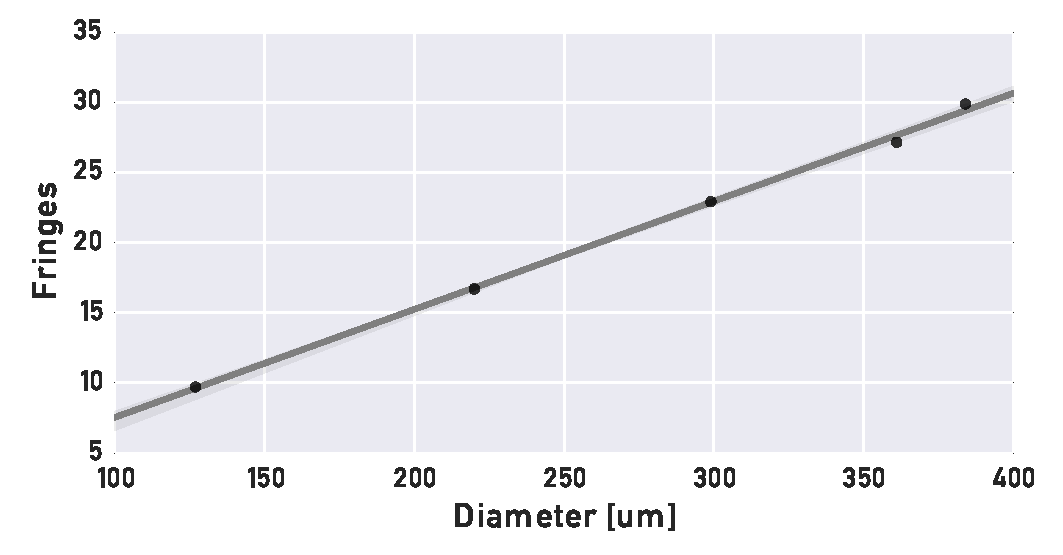
\includegraphics[width=0.8\textwidth]{img/fringe_regression.pdf}
    \caption{Scatterplot of \tableref{tab:ipi-calibration-datasets} showing the peak fringe counts $\hat{N}_\text{fr}$ for each predicted droplet diameter $D_d$}
    \label{fig:fringe-regression}
\end{figure}
It must be remembered, of course, that the peak fringe count values
$\hat{N}_\text{fr}$ forming the basis of our calculation are taken from the
peaks of Gaussians fitted to the raw fringe count histograms (see
\figref{fig:fringe-histograms}. In other words, it is our assumption that all
droplets from a given dataset produce fringe counts that are normally
distributed around their respective $\hat{N}_\text{fr}$. The histogram to
dataset FA shows a much higher deviation than the others -- this may be due to
genuine variance in the generated droplet diameters or to difficulty in
processing comparatively weak images with low fringe counts. It seems likely
that both effects contribute.

We can compare the empirically determined value $\hat{\kappa}$ with the
mathematical result obtained from \eqref{kappa}. Substituting $\lambda = 532$
nm, $m = 1.3324$ and $\phi = 90^\circ$, we conclude that
\begin{equation}
    \frac{D_a}{z} = 2 \sin \left( \frac{\hat{\kappa} \lambda}{\cos
    \frac{\phi}{2} - \frac{ m \sin \frac{\phi}{2}}{\sqrt{m^2 + 1 - 2m \cos
    \frac{\phi}{2}}}} \right) = 2\sin (3.11982 \cdot 10^{-7} \hat{\kappa})
\end{equation}
so for $\hat{\kappa} = 76808.1$, $\frac{D_a}{z} = 0.047921$. Recall that this
quotient is a measure of the collection angle and closely related to the
numerical aperture NA$=\sin \frac{D_a}{2z}$. If needed, we can now use this
result to compute the input parameters $D_a$ and $z$ in the DantecStudio IPI
software: given, for instance, $z = 45.0$ cm, we can obtain the entrace pupil
diameter as
\begin{equation}
    0.047921~\cdot~450\,\mathrm{mm} = 2.156\,\mathrm{mm}
\end{equation}


\section{Removing center discrepancies with keypoint registration}
\label{sec:keypoint-registration}

%TODO: Say that the bulk of the following work is from Kosch and Ashgriz,
%submitted to journal/conference XYZ
As mentioned above, to allow both cameras to image the same physical region in
the spray, they are either placed behind a beamsplitter at a right angle to the
light sheet, or placed separately at different angles. The latter approach makes
for a more difficult setup, since Scheimpflug's rule demands that the camera
must be tilted with respect to the objective lens, but it gives the user the
freedom to choose the highest-intensity scattering angle.

In any of the above cases, the use of two cameras requires that their images be
mapped onto one another. This is commonly achieved by means of a camera
calibration procedure, in which a target pattern (e.g. as in \figref{fig:plate-calibration}) of known dimensions is
photographed by each camera. A pattern recognition algorithm then determines the
object-to-image mappings for each camera:


\begin{equation}
\left[\begin{array}{c} x'\\ y'\\ z'\\ r' \end{array} \right]
=
\left[ \begin{array}{cccc}
S_x & A_{yx} & A_{zx} & T_x \\
A_{xy} & S_y & A_{zy} & T_y \\
A_{xz} & A_{xy} & S_z & T_z \\
P_x & P_y & P_z & S_0
\end{array} \right]
\left[ \begin{array}{c} x\\ y \\ z \\ 1 \end{array} \right].
\end{equation}
\begin{figure}
    \centering
    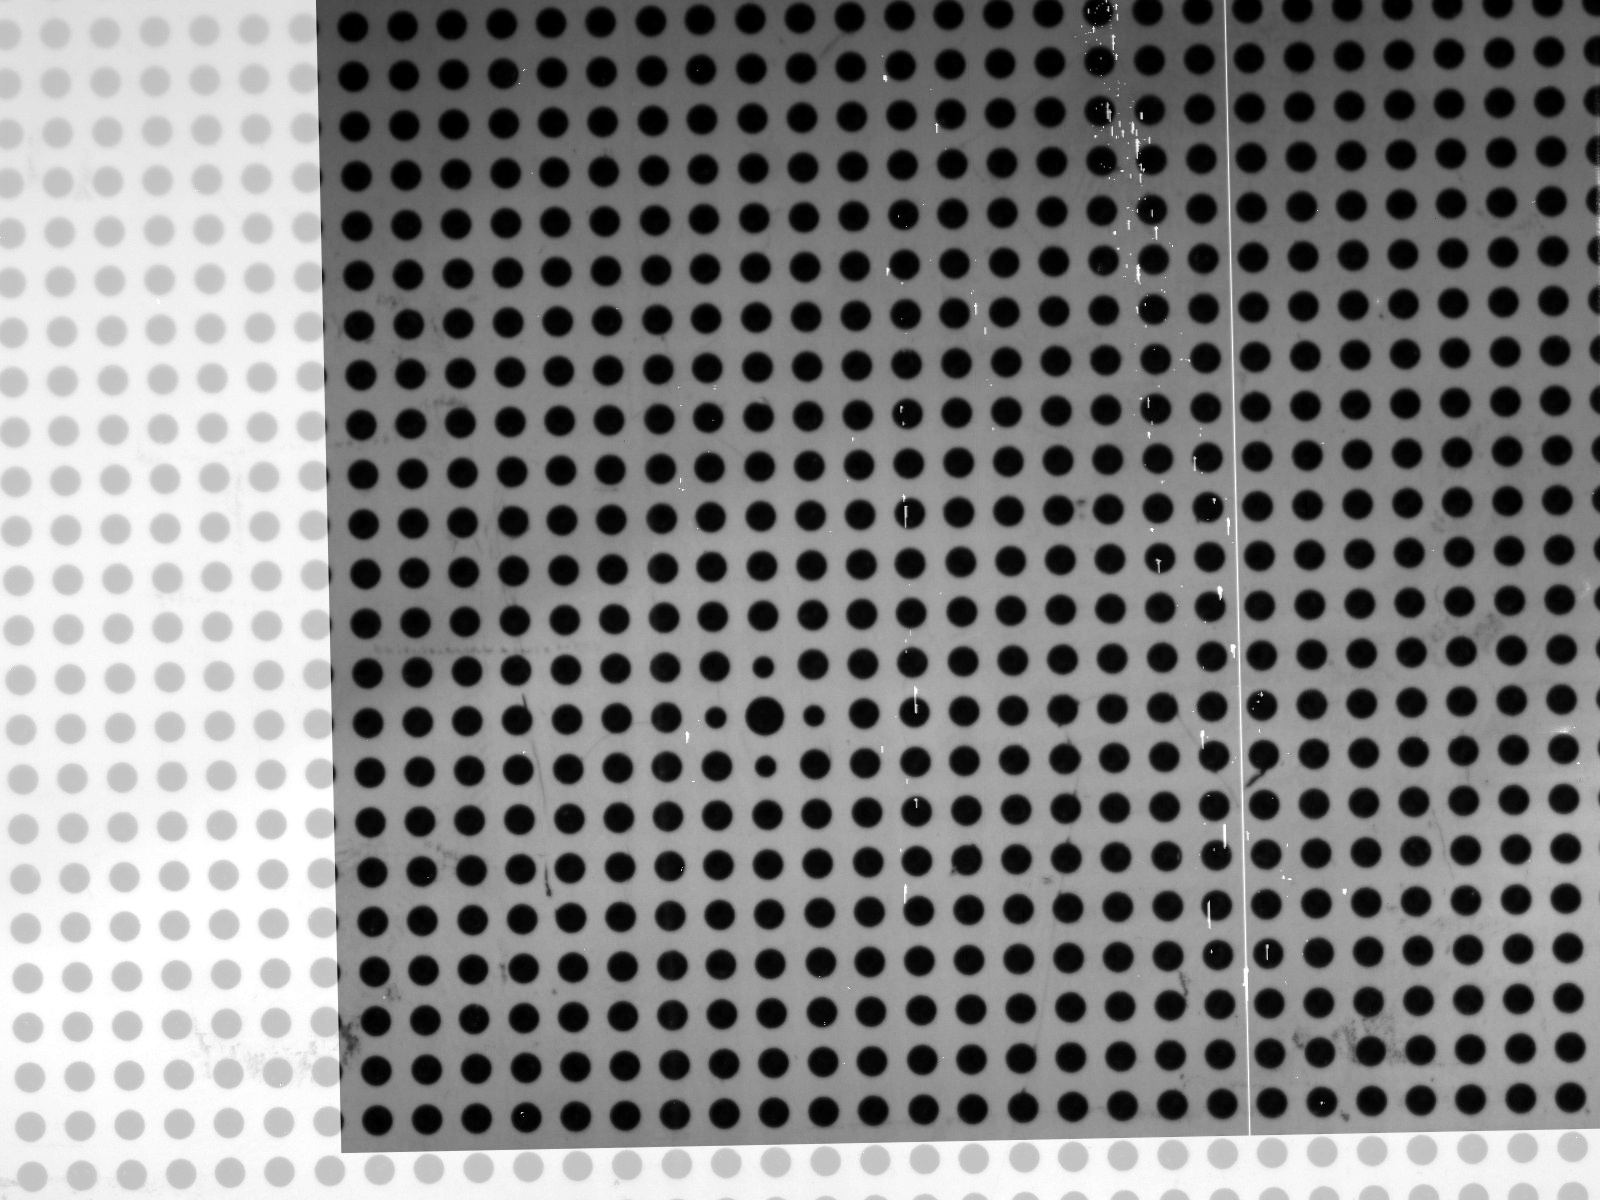
\includegraphics[height=0.45\textheight]{img/orb/plate-calibration.jpg}
    \caption{Homography $\mathbf{H}$ applied to target pattern image captured by
        the focused camera and superimposed on the image captured by the
        defocused camera (here, both cameras were in focus for the calibration
        only).
    \label{fig:plate-calibration}}
\end{figure}

In our case, Dantec supplied a \emph{standard dot target}, a white $10 \times 10\,
\mathrm{cm}^2$ plate engraved with a pattern of black dots. The plate is to be
mounted such that its surface coincides perfectly with the laser sheet. 

In practice, $P_{x,y,z} = 0$ and $S_0 = 1$ is assumed, such that the mapping is
affine. The $z$-components (third row/column) are further assumed to be zero,
such that a $3 \times 3$ matrix suffices for the purposes of this discussion:
\begin{equation}
\left[\begin{array}{c} x'\\ y'\\ r' \end{array} \right]
=
\left[ \begin{array}{ccc}
S_x & A_{yx} &  T_x \\
A_{xy} & S_y &  T_y \\
P_x & P_y & S_0
\end{array} \right]
\left[ \begin{array}{c} x\\ y \\ 1 \end{array} \right].
\end{equation}

The calibration algorithm thus finds the camera matrices
$\mathbf{P}_\text{foc}$ and $\mathbf{P}_\text{def}$ mapping the
object coordinates $\mathbf{x}$ onto the two camera images
$\mathbf{x}_\text{foc}'$ and $\mathbf{x}_\text{def}'$ (the respective 
    subscripts shall hence designate the focused and defocused
    cameras):
\begin{align}
    \mathbf{x}_\text{foc}' &= \mathbf{P}_\text{foc} \, \mathbf{x} \\
    \mathbf{x}_\text{def}' &= \mathbf{P}_\text{def} \, \mathbf{x}.
\end{align}

It follows that the quotient of the two matrices, also known as the homography
\begin{equation}
    \mathbf{H} = \mathbf{P}_\text{def} \, \mathbf{P}_\text{foc}^{-1}
\end{equation}
can be used to map the focused image onto the defocused image, as shown in \figref{fig:plate-calibration}:
\begin{equation}
    \mathbf{H}\, \mathbf{x}_\text{foc}' = \mathbf{x}_\text{def}'.
    \label{homography-definition}
\end{equation}
Unfortunately, the calibration procedure itself introduces an unwanted
distortion: to capture a viable photo of the target pattern, the defocused
camera must be temporarily brought into focus, as was done in
\figref{fig:plate-calibration}. This is not mentioned e.g. in the
application manual of Dantec's IPI system, but is a practical necessity.
Bringing a camera out of focus not only introduces a blur, it also scales the
image extents. \figref{fig:discrepancy}, adapted from \citet{Hardalupas10},
shows schematically how this effect creates ``center discrepancies''. Since the
extents of the defocused image are either smaller or larger than those of the
focused image, depending on the direction of defocusing, all droplet images are
projected either closer to or farther away from the image center. The
discrepancy is worst for droplets far away from the image center. As a result,
the centers of objects in simulatenously captured focused and defocused images
no longer align (\figref{fig:drop-calibration-off}), and the calibration
procedure becomes self-defeating.

\begin{figure}
\centering
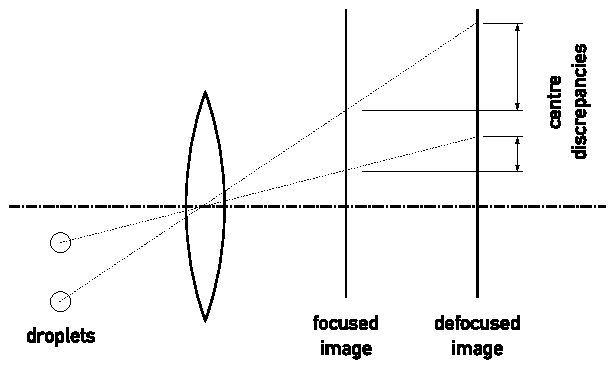
\includegraphics[width=0.7\textwidth]{img/orb/discrepancy.pdf}
\caption{Schematic showing the source of center discrepancies in the case of
parallel image and object planes \label{fig:discrepancy}}
\end{figure}

\begin{figure}
    \centering
    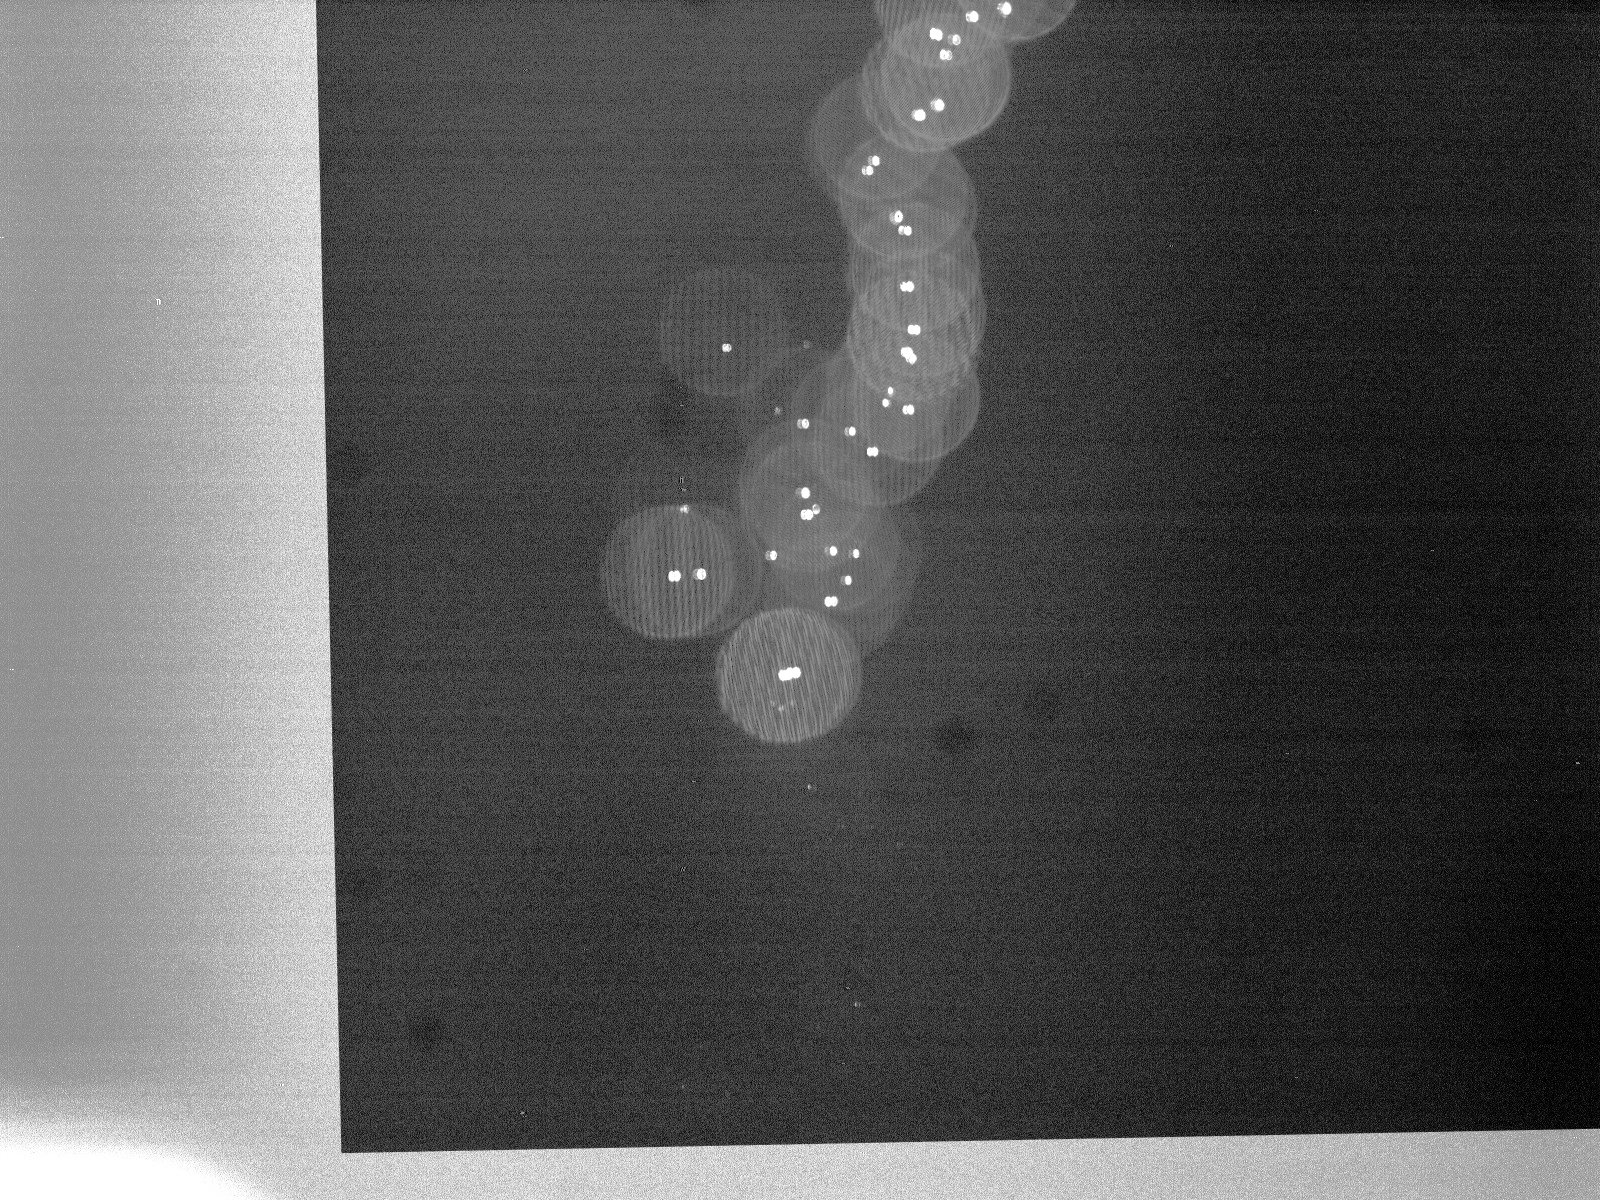
\includegraphics[height=0.45\textheight]{img/orb/drop-calibration-off.jpg}
    \caption{Focused camera image, after applying homography $\mathbf{H}$
        derived from the calibration images, is superimposed onto
    defocused camera image of droplets. Discrepancies between object centers
grow towards the edge of the image.}
    \label{fig:drop-calibration-off}
\end{figure}

While this error is easy to account for in the ideal case of right angles and
perfect alignments (simply rescaling the image would solve the problem) the
situation becomes more difficult in practice when the target pattern is no longer
parallel to the camera sensor (intentionally or accidentally) or when
cylindrical lenses are used to add optical compression. In fact, there is no
guarantee that affine mappings are sufficient in the general case.

Surprisingly, only Hardalupas~\emph{et al.} \cite{Hardalupas10, Hardalupas10a}
have hitherto published a discussion of this effect, and the only previous
mention known to the authors is in \citet{Kurosawa02}, who dismissed it as a
``positioning error''.

Hardalupas \emph{et al.} identified the centers of particles in both PIV
(focused) and ILIDS (defocused) images. They then empirically estimated the
magnitude of the center discrepancy effect along the vertical axis, which
enabled them to improve the accuracy of their nearest-neighbour-based droplet
image matching algorithm.

We found that algorithms developed by the computer
vision community in recent years can obviate the need for calibration entirely.
Instead, we can use visual correspondences between the focused and defocused
images to find the mapping between them directly. To that end, we first provide
in \secref{sec:keypoint-review} a brief overview over popular methods in the field of automated (linear)
\emph{registration}, i.e. the art of finding a \emph{homography} (geometric
mapping) between two \emph{epipolar images} (images of the same object, taken
from different positions and angles). \secref{sec:keypoint-results} documents 
our approach in greater detail and shows the result of a successful
recalibration.

\subsection{Review of image registration techniques \label{sec:keypoint-review}} Given two
identical images that have been rotated, shifted or even scaled with respect to
one another, the applied transformation can theoretically be found by means of a
brute-force search. This method is not feasible in practice, not only because of
its enormous computational complexity (there are no gradients to guide the
search) but also because of its inability to deal with noise, focal blur,
perspective changes and other nonlinearities introduced by the photographic
process. Conversely, normalized cross-correlation measures between images, as
commonly used in PIV, are unaffected by noise but not invariant to rotation and
scale and therefore not generally practical. The standard approach to image
registration is therefore a three-step process. First, \emph{keypoints}, i.e.
``interesting'' points in the images are found by a keypoint detection
algorithm.  Then, a small image patch at every keypoint is extracted and
converted into a \emph{feature vector}, a set of numbers providing a very
general description of the image patch that accounts for scale, rotation, blur,
contrast, etc. Finally, matches between similar feature vectors from the two
images are found, outliers are removed, and the homography is calculated.

However, the results of a keypoint detection algorithm
must be as repeatable as possible, i.e. the same set keypoints should be found
in both images regardless of their relative position, rotation, scale, etc. 
For instance, the Harris corner detector \cite{Harris88}, one of the earliest
keypoint detectors, is sensitive to scale and thus often unusable.

The recent decade has seen a rapidly growing collection of proposed keypoint detectors,
beginning with \textsc{sift} \cite{Lowe04}, \textsc{surf} \cite{Bay08} and
\textsc{brisk} \cite{Leutenegger11}, all of which include keypoint extractors, to
\textsc{censure} \cite{Agrawal08}, optimized for speed, and
\textsc{fast} \cite{Rosten05}, which incorporates machine learning methods.
Finally, the recent publication of \textsc{orb} \cite{Rublee11} includes a
rotation-aware version of \textsc{fast} used in this paper. Many more have been
developed but are not included here for brevity's sake.

Keypoint extractors (sometimes called \emph{descriptors}) are often optimized
for and therefore included with keypoint detectors, as in the instances
mentioned above. Some however are standalone algorithms, such as
\textsc{brief} \cite{Calonder10}.

It is straightforward to find matching keypoints by searching for pairs
with the smallest arithmetic distance between their feature vectors (e.g. using the $L^2$ norm). This nearest-neighbour search
can be done exhaustively in linear time to find the optimal matching, but many
faster, if approximate, search methods exist. We should note \textsc{flann} \cite{Muja09},
a publicly available collection of such implementations which includes a fully
automatic parameter selection heuristic.

Finally, the homography, assuming one exists, can be derived from the set of
matched keypoint coordinate pairs. Since many of the found matches will be
wrong, it is of essence to use a robust estimator, i.e. a type of regression
model designed to ignore outliers. Possibly the oldest of these methods is
\textsc{ransac} \cite{Fischler81}, an iterative procedure in which sets of data points are
chosen at random and discarded if the agreement between a model fit to them and
all other data points falls below a carefully chosen threshold. \textsc{ransac} was used
for this paper, although other robust methods exist. The criterion developed by
\citet{Moisan04} deserves special mention in our context; it does away with
\textsc{ransac}'s hard threshold and instead takes into consideration the probability of
a match to be in consensus with epipolar geometry.

\subsection{Using affine oriented \textsc{fast}, \textsc{brief} and \textsc{ransac} to estimate the homography
between PIV and ILIDS photographs \label{sec:results}}

Existing PIV/ILIDS systems derive the homography from the result of a camera
calibration procedure which the user is required to perform before analyzing
images.
Although the final value of $\mathbf{H}$ is invisible to the user in our copy of
Dantec's DynamicStudio software, the camera matrices $\mathbf{P}_\text{foc}$ and
$\mathbf{P}_\text{def}$ can be shown and edited. We therefore must find a
corrected homography $\mathbf{\hat{H}}$ that allows us to compute
\begin{equation}
    \mathbf{\hat{P}}_\text{def} = \mathbf{\hat{H}} \, \mathbf{P}_\text{foc}
    \label{corrected-homography-use}
\end{equation}
so that we can replace $\mathbf{P}_\text{def}$ with $\mathbf{\hat{P}}_\text{def}$ in
the software, effectively correcting $\mathbf{H}$ to $\mathbf{\hat{H}}$.

To efficiently extract keypoints, we combined three algorithms:
\textsc{asift} \cite{Morel09} to deal with skew transformations; an oriented version of
\textsc{fast}, published as part of \textsc{orb}, to detect keypoints; and
standard \textsc{brief} as a keypoint extractor.

\textsc{asift} is a method originally developed to be used with \textsc{sift}.
It introduces invariance to affine mappings by simulating various
projective transformations while \textsc{fast} and \textsc{brief} are run repeatedly.
This slows the analysis down, but given the infinitude of
possible angled camera-camera-object configurations, it is wise to maintain a
flexible framework.

We should note that the original \textsc{asift} with
\textsc{sift} works well, but \textsc{sift} is encumbered by patents. To
encourage vendors of imaging systems to adopt the proposed algorithms, we made
it our goal to find a freely available replacement.

Recall that the disks in the defocused image are missing from the focused image,
rendering a registration between them impossible. It is straightforward to
simulate the disks, however. We followed the following protocol on our focused
images:
\begin{enumerate}
    \item Mask the image, blacking out all areas that are known not to contain
        droplets.
    \item Subtract the pixel-wise minimum or mean value taken over all images
        taken by the camera. This step serves to black out defective hot pixels
        on the camera's CCD and other static noise.
    \item Erode the image, using a $3\times 3$ or $5\times 5$ kernel. This will
        close any remaining bright pixels which are likely noise.
    \item Locate the intensity peaks in the remaining image.
    \item Fill a blank image with black, then draw bright circles of diameter
        $D_\text{disk}$ onto it, centerd at the respective positions of the
        intensity peaks detected in the focused image. (Note that simply dilating
        the result of the previous step will not lead to circular disks.)
\end{enumerate}
\begin{figure}
    \centering
    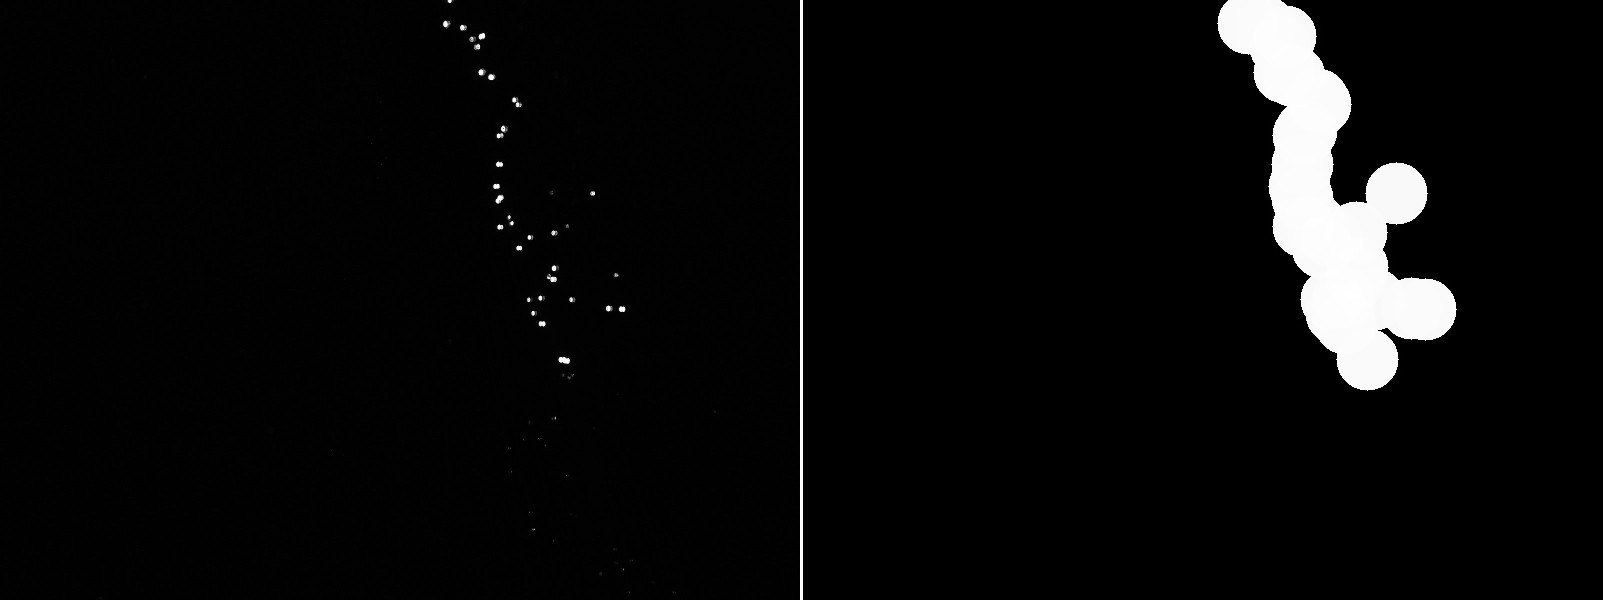
\includegraphics[width=\textwidth]{img/orb/dilation.jpg}
    \caption{Simulating disks based on the focused image. \label{fig:making-disks}}
\end{figure}

The result of performing these operations on our sample image is shown in \figref{fig:making-disks}. We determined the disk diameter $D_\text{disk}$
empirically from the defocused images, although it is naturally preferable to
automate this step, e.g. using circular Hough transforms or cross-correlation
with circular masks. There may be simpler ways of achieving the same result,
e.g. by means of Gaussian filters, distance transforms and thresholding
operations. However, we found the protocol described above to be quite robust to
noise and fast enough for our application.

Implementations of \textsc{orb} and \textsc{brief} are freely available through
the OpenCV project, which provides bindings for the C++ and Python languages. We
used these implementations to find and extract matching keypoints between our
sample images, shown in \figref{fig:matching}.

\begin{figure}
    \centering
    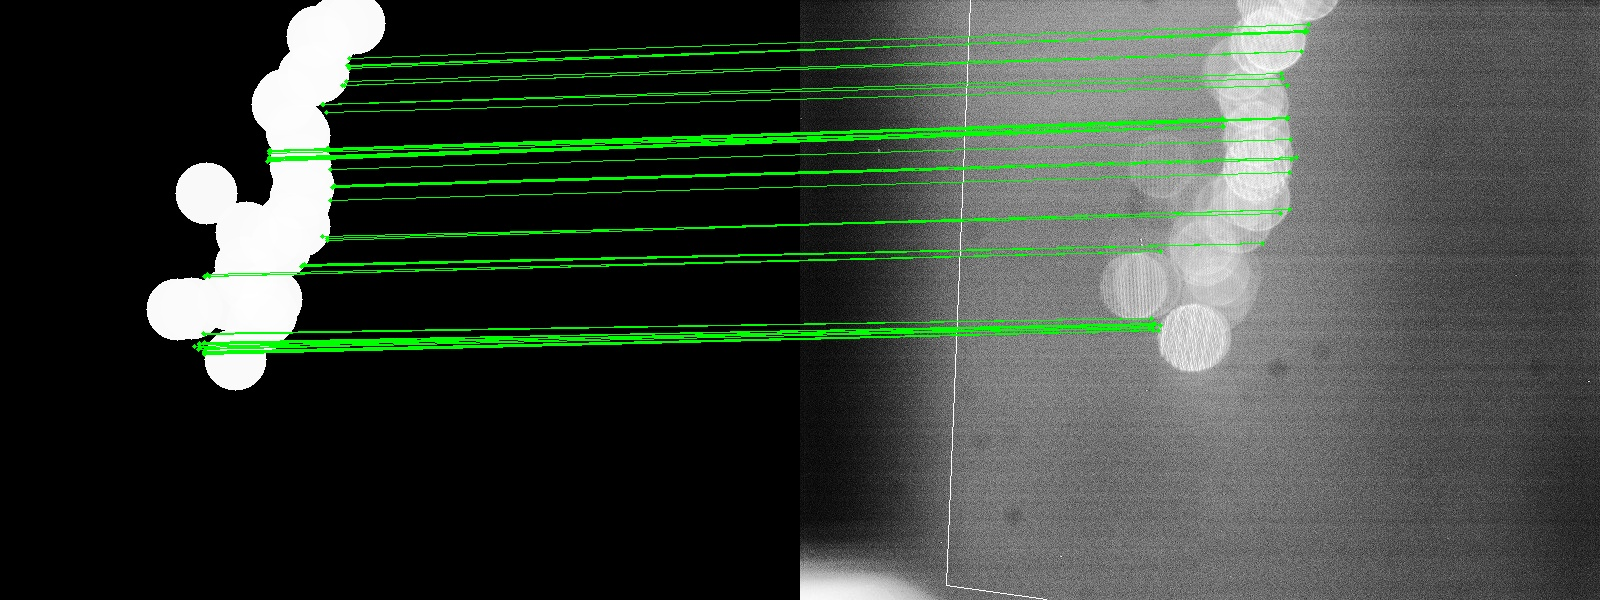
\includegraphics[width=\textwidth]{img/orb/asift-matching.jpg}
    \caption{Visualized inliers in the set of matched keypoints between the
    mirrored simulated disks (see \figref{fig:making-disks}) and the ILIDS image. \label{fig:matching}}
\end{figure}

The matches shown in \figref{fig:matching} were found using a most basic
method: brute-force match search, followed by a \textsc{ransac} estimation of the
homography matrix $\mathbf{K}$ using a threshold of 10.

Since the two cameras were positioned behind a beamsplitter in our setup, the
defocused image was flipped horizontally. We therefore first mirrored it
horizontally, using the transformation matrix
\begin{equation*}
    \mathbf{M}_h = \left[ \begin{array}{ccc}
    -1 & 0 & \text{(image width)} \\
            0 & 1 & 0 \\
            0 & 0 & 1
    \end{array} \right].
\end{equation*}
To speed up the image registration process, it can be helpful to first down-scale the
images. To reduce an image to half of its original size, apply
\begin{equation*}
    \mathbf{S}_{0.5} = \left[ \begin{array}{ccc}
    0.5 & 0 & 0 \\
            0 & 0.5 & 0 \\
            0 & 0 & 1
    \end{array} \right].
\end{equation*}
While the above operations might not be strictly necessary, we found that they
significantly improved the quality of the matches identified.
If the registration algorithms mentioned above now find a homography matrix
$\mathbf{K}$, then we can write
\begin{equation}
    \mathbf{K}\, \mathbf{M}_h\, \mathbf{S}_{0.5}\, \mathbf{P}_\text{foc} =
    \mathbf{S}_{0.5} \mathbf{P}_\text{def}
\end{equation}
and to bring this into a form similar to \eqref{homography-definition}, 
\begin{align}
    \mathbf{S}_{0.5}^{-1}\, \mathbf{K}\, \mathbf{M}_h\, \mathbf{S}_{0.5}\,
    \mathbf{P}_\text{foc} &=
     \mathbf{S}_{0.5}^{-1}\, \mathbf{S}_{0.5} \mathbf{P}_\text{def} \\
     &= \mathbf{P}_\text{def}
\end{align}

Finally, it turns out that Dantec's DynamicStudio software violates convention
by placing the coordinate origin at the bottom (not top) left corner of the
image. We must therefore pre- and post-multiply by $\mathbf{M}_v^{\pm 1}$, with
\begin{equation*}
    \mathbf{M}_v = \left[ \begin{array}{ccc}
            1 & 0 & 0 \\
    0 & -1 & \text{(image height)} \\
            0 & 0 & 1
    \end{array} \right],
\end{equation*}
to arrive at our final expression for $\mathbf{\hat{H}}$:
\begin{equation}
    \mathbf{\hat{H}} = \mathbf{M}_v\, \mathbf{S}_{0.5}^{-1}\, \mathbf{K}\,
    \mathbf{M}_h\, \mathbf{S}_{0.5}\, \mathbf{M}_v^{-1}.
\end{equation}
Substitution of $\mathbf{\hat{H}}$ into \eqref{corrected-homography-use} yields
$\mathbf{\hat{P}}_\text{def}$, which can be manually entered into the
DynamicStudio software. \figref{fig:drop-calibration-corrected} illustrates
how the use of $\mathbf{\hat{H}}$ leads to an improved alignment compared to
\figref{fig:drop-calibration-off}. Note that a slight projective distortion
is necessary for optimal registration, confirming that it is infeasible to restrict the homography
to affine matrices.

\begin{figure}
    \centering
    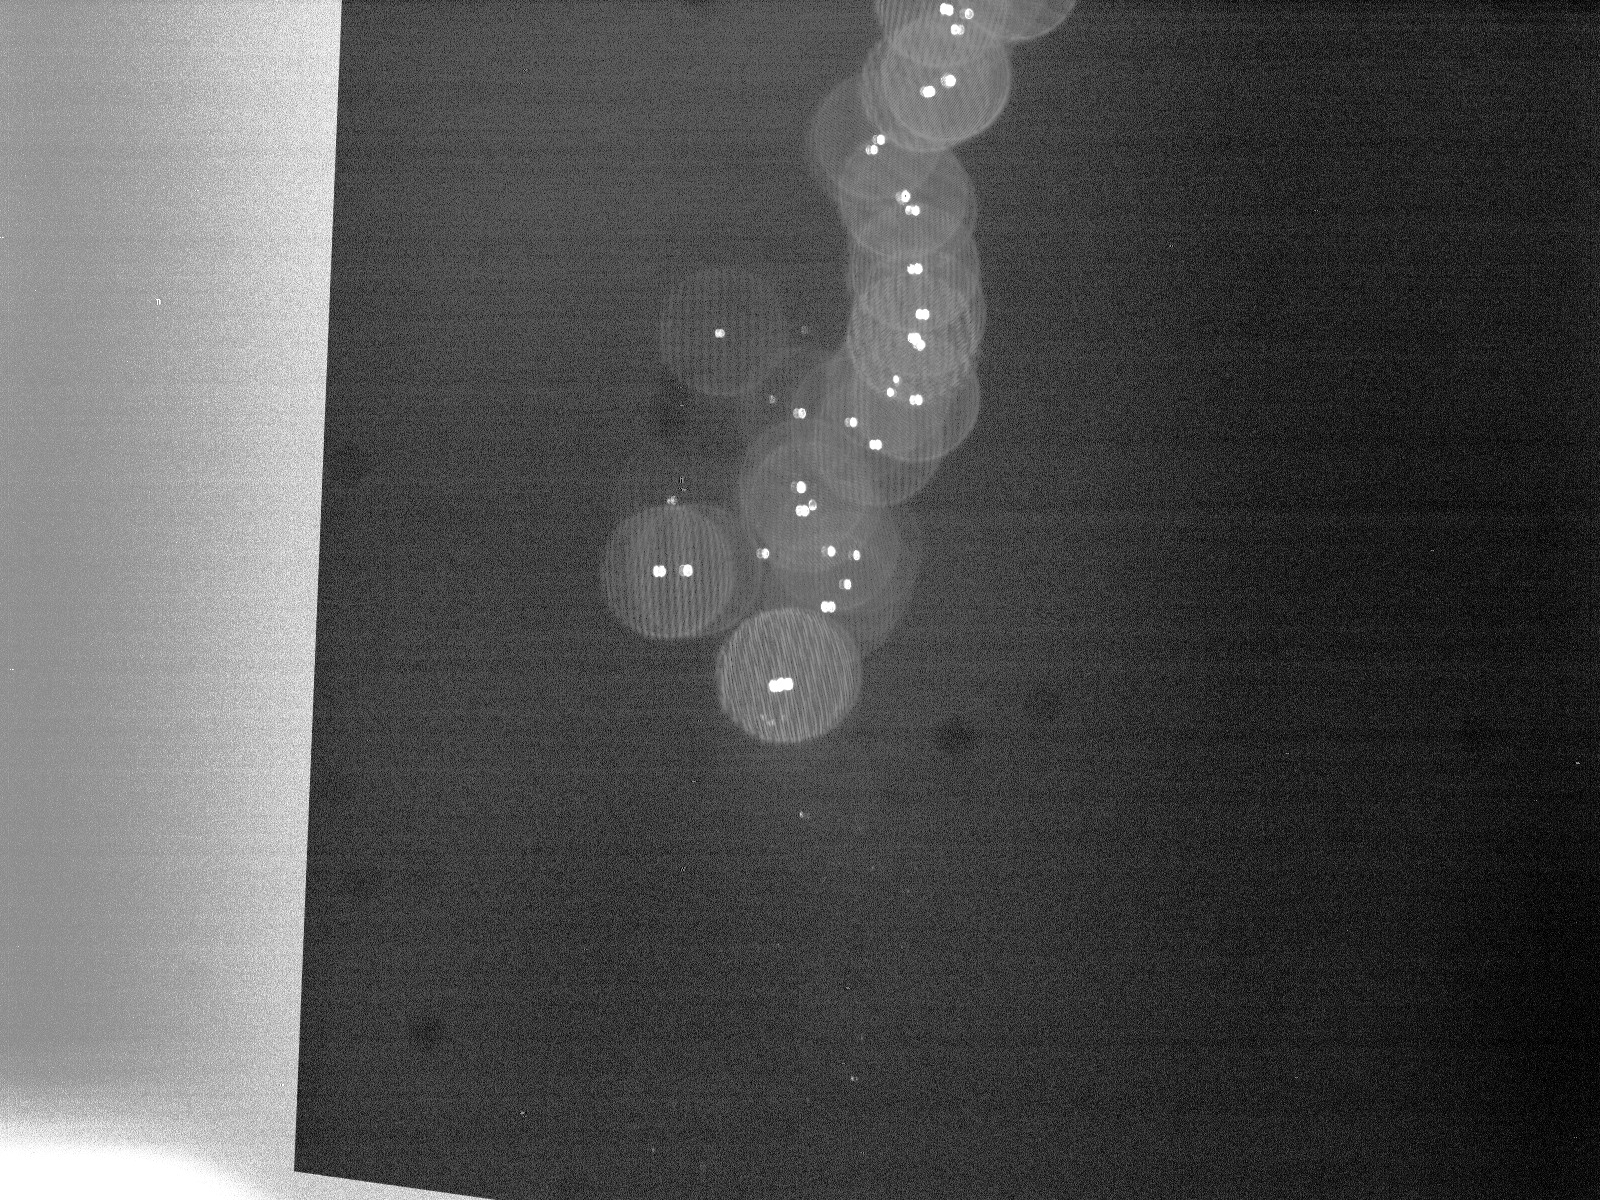
\includegraphics[height=0.45\textheight]{img/orb/drop-calibration-corrected.jpg}
    \caption{Focused camera image, after applying corrected homography
        $\mathbf{\hat{H}}$ derived from the matched keypoints, is superimposed onto
    defocused camera image of droplets.}
    \label{fig:drop-calibration-corrected}
\end{figure}

\section{Removing center discrepancies with point set registration}
\label{sec:point-set-registration}
The keypoint matching approach described above is not applicable when a slit
aperture was used to reduce overlap, as in the paper by Hardalupas
\emph{et~al.}, so we will outline briefly how to use registration algorithms
with such setups.\footnote{While slit strip images could be
simulated over the focused image (in a procedure analogous to that illustrated
in \figref{fig:making-disks}), the lack of overlap between them could make it
significantly more difficult to find ``interesting'' keypoints in the simulated
image.}

Keypoints are not required, when the absence of overlap allows
us to identify focused and defocused objects centers directly from the respective
images and find a projection mapping between them. Indeed, Hardalupas
\emph{et~al.} successfully registered their PIV and ILIDS images that way: using
wavelet transforms at various frequencies, they identified the putative droplet
centers on both focused and defocused images.  Then, using a continuous,
single-stream monodisperse droplet generator, they estimated how the magnitude
of the center discrepancies varied over the image.  After applying this
empirically estimated distortion to the captured focused images, they matched each
focused droplet to the closest defocused droplet (if one could be found within an
subjectively chosen search distance).

Although they reported good success using this method, it requires both an
empirical estimation of the center discrepancies every time the camera is
defocused \emph{and} a guess at the appropriate search window size. Moreover,
mismatches are likely as the naive closest-neighbour search is not robust to
noise. To eliminate these steps, we suggest that droplet matches be found
directly using a robust point set registration algorithm.

Since the early 1990s, computer vision researchers have accumulated an
impressive body of work on this topic, most of it focusing either
on rigid transformations (i.e. translation and rotation only) or non-rigid
transformations (typically understood to include nonlinear warping). The problem
at hand requires an algorithm able to deal with projective transforms, which
are non-rigid but linear.

The only paper known to the authors to specifically address this case is by
\citet{Chi11}, who propose an iterative search based on image moments. Since
image moments are an aggregate metric, they do not directly lead to a
droplet-to-droplet correspondence. Still, closest-neighbour matches after
application of this algorithm would likely produce results no worse than those
found after estimating the transformation empirically.

Robust non-rigid methods are also applicable in this case and deserve some
mention. Many of them are probabilistic relaxations of the Iterative Closest
Point algorithm, which simply searches for the least-squares-optimal rigid
mapping. Several of these approaches were reviewed and generalized by
\citet{Jian10}. A slightly different approach, named Coherent Point
Drift\cite{Myronenko10}, is also highly popular and illustrated in \figref{fig:cpd}.
\begin{figure}
    \centering
    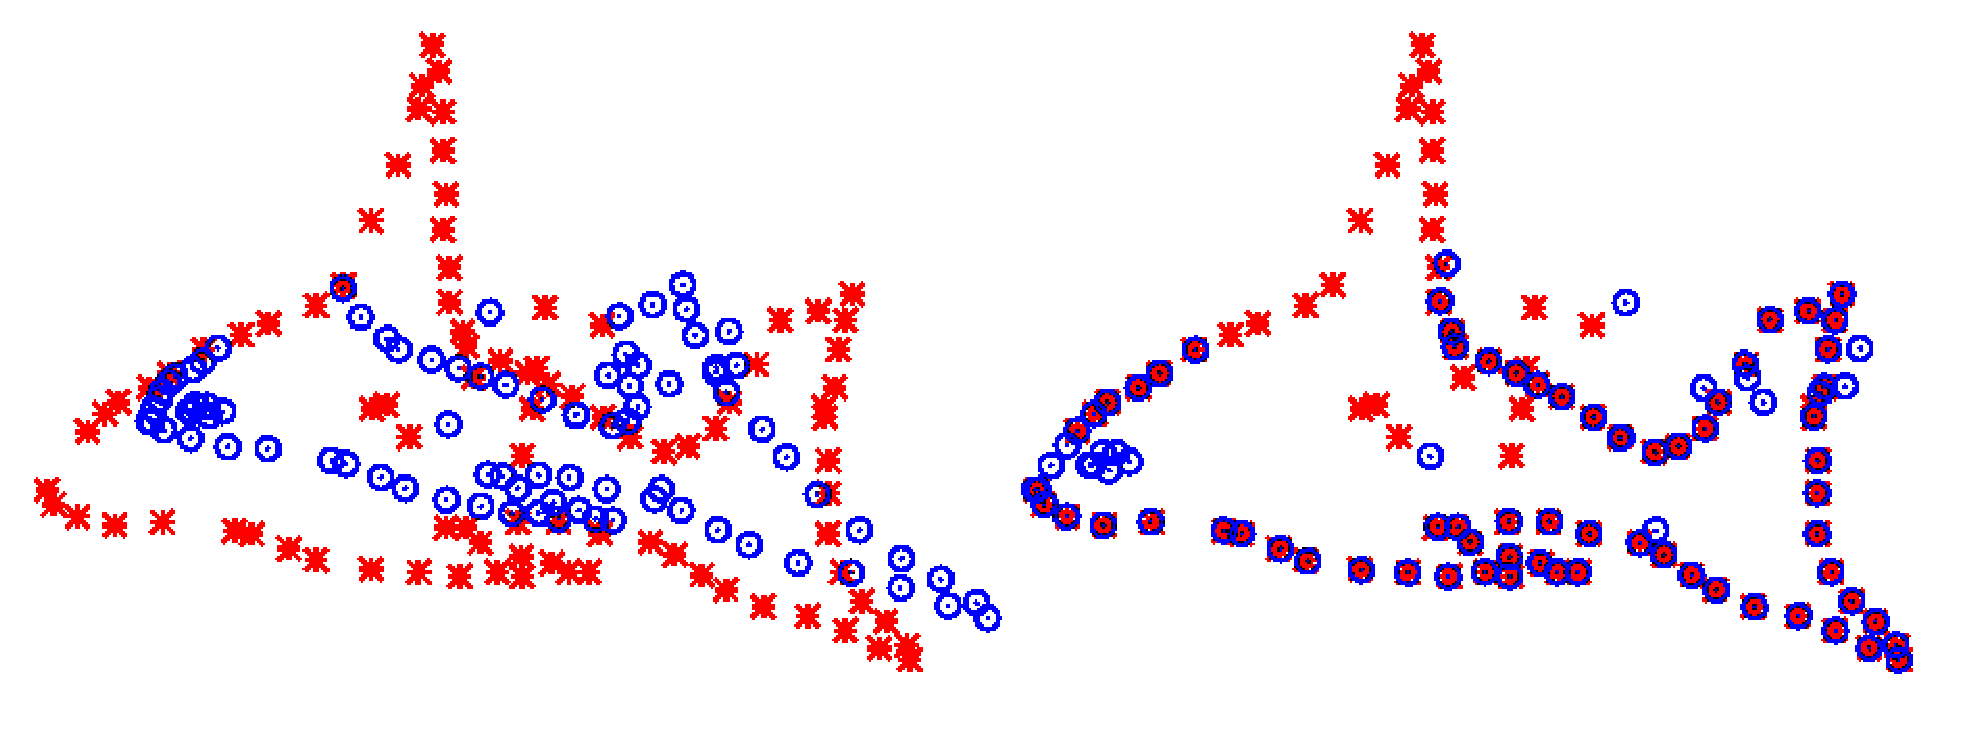
\includegraphics[width=0.8\textwidth]{img/orb/pointset.eps}
    \caption{Non-rigid variant of the Coherent Point Drift algorithm applied to
    two point sets. Notice that the probabilistic nature of the matching creates
robustness to unmatched points. (Image source: Wikipedia)}
    \label{fig:cpd}
\end{figure}

We forgo at this point a documentation of the application and refer the reader to
Hardalupas \emph{et al.}, who describe their center identification technique in
good detail, and to the above-mentioned authors, who have published freely
available implementations of their algorithms online.

%%%%%%%%%%%%%%%%%%%%%%%%%%%%%%%%%%%%%%%%%%%%%%%%%%
%%%%%%%%%%%% PDPA %%%%%%%%%%%%%%%%%%%%%%%%%%%%%%%%
%%%%%%%%%%%%%%%%%%%%%%%%%%%%%%%%%%%%%%%%%%%%%%%%%%

\chapter[Phase-Doppler Particle Analysis]{Phase-Doppler\\Particle Analysis (PDPA)}
Phase-Doppler anemometry and droplet sizing techniques are based on the
far-field intensity fluctuations in the laser light scattered by passing
droplets. Unlike ILIDS, however, PDPA uses intersecting laser beams (instead of
a laser sheet) to illuminate the droplets. Whereas ILIDS \emph{images} the
infringement pattern cast by the glare points on the illuminated droplet, PDPA
measures the fringe spacings indirectly by relating them to the phase difference 
between the signals recorded by a pair of adjacent detectors. 

\citet{Doppler42} suggested in 1842 that the slight differences in wavelength between
the colours of various stars could be used to determine the stars' velocities relative to
Earth. A century later, military radar operators during World War II realized that the Doppler
effect could be exploited to estimate target velocities using their radar
systems. Soon, meteorologists had adopted the technology to measure wind speeds
\cite{Whiton98}. The flurry of activity around Doppler measurements in the
ensuing years produced the first laser-based particle anemometry system,
designed in 1964 by \citet{Yeh64}, and several novel beam-detector
configurations have been proposed since. Among them are the popular dual-beam
configurations, constitutiting a departure from the original reference beam
systems which can be more difficult to align. A exemplary dual-beam setup is
shown in \figref{fig:pdpa-setup}.

\begin{figure}
    \centering
    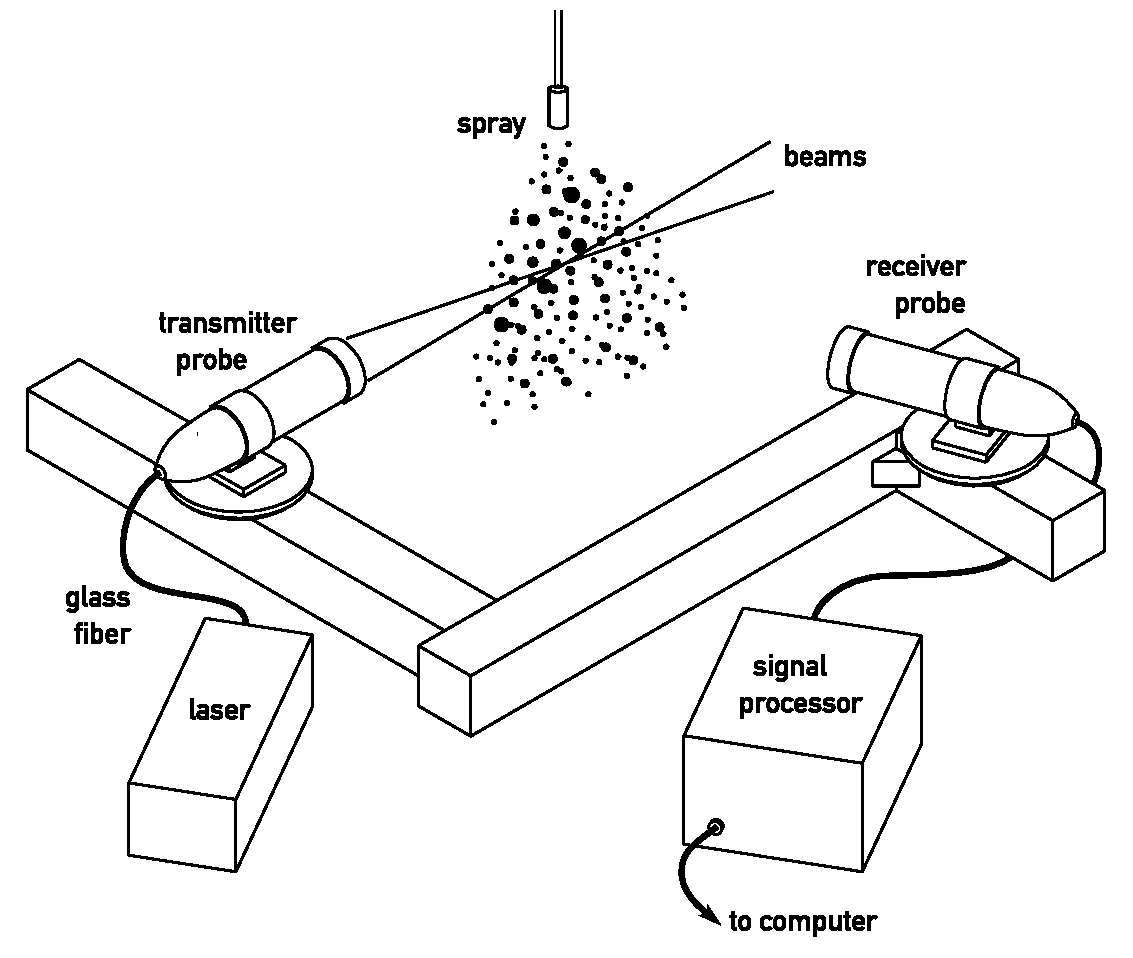
\includegraphics[width=0.75\textwidth]{img/setup/pdpa_setup.pdf}
    \caption{Typical commercial PDPA configuration using transmitter and
        receiver probes \label{fig:pdpa-setup}}
\end{figure}

Laser-Doppler anemometry (LDA, also known as laser-Doppler velocimetry or LDV)
provides velocity measurements only. The 1970s saw the discovery that the fringe
patterns cast by the scattered light could be analyzed to yield size information
\cite{Durst76, Wigley78}. This technique is now widely used and often
integrated into the detecting and processing hardware of commercial LDA systems,
typically under the name of phase-Doppler Anemometry (PDA) or phase-Doppler
particle analysis (PDPA).

PDPA can be used to ascertain droplet size distributions with a very high
precision. Nevertheless, its accuracy hinges on the knowledge of a large number
of distances, angles and voltages. A single erroneous one of them will throw
off the result, leaving the operator none the wiser. We shall therefore discuss
briefly the various sources of error in this chapter, and provide some pointers
to their resolution. The focus is on measurements of size, not velocity.

\section{Optical principle}
Only droplets passing through the measurement volume have a chance of being
detected and characterized, so we will provide here a description of the 
measurement volume and its interaction with a falling droplet.

To create the measurement volume, two laser beams must intersect where their
wave fronts are planar. To this end, the transmitter probe features a front lens
which focuses the beams to a small but finite \emph{waist diameter}. Note that
focusing onto an infinitesimally small point is impossible: as the beam is
exiting from a finite-sized aperture, some degree of diffraction is unavoidable
and will lead to a finite diameter. In the case of most commercial setups, the
laser exhibits a Gaussian intensity profile, i.e. the light intensity falls off
smoothly with increasing distance from the beam axis. The diffraction of a
Gaussian beam generally causes spherically expanding wavefronts
\cite{Thyagarajan10}; the focusing lens counteracts this effect and leads to
plane waves at the beam waist.

Borrowing from the terminology used by \citet{Albrecht03}, the \emph{measurement
volume} is the space in which a particle must be located such that it scatters
the light onto the detector. For large particles, this will not coincide
perfectly with the illuminated volume. The measurement volume contains the
\emph{detection volume}, within which a droplet scatters enough light onto the
detector to exceed the chosen minimum threshold for detection.

In accord with most introductory texts on PDPA, we will offer two descriptions
of the scattering effect experienced by the droplets falling through the
measurement volume: a fringe model for very small droplets, and a Moiré model
for larger droplets.

\subsection{Particles smaller than the wavelength}
The intersection of the two beams results in their interference at an angle
$\Theta$. The alternating extinction and amplification creates a pattern of
fringes. As the small droplet (assumed to be a single point) falls through the
fringes, it samples the light intensity, scattering an alternating signal onto
the detector, which registers a burst of voltage spikes. Since the fringe
spacing is known and constant, the detected burst frequency is linearly related
to the velocity of the falling droplet.

\begin{figure}
    \centering
    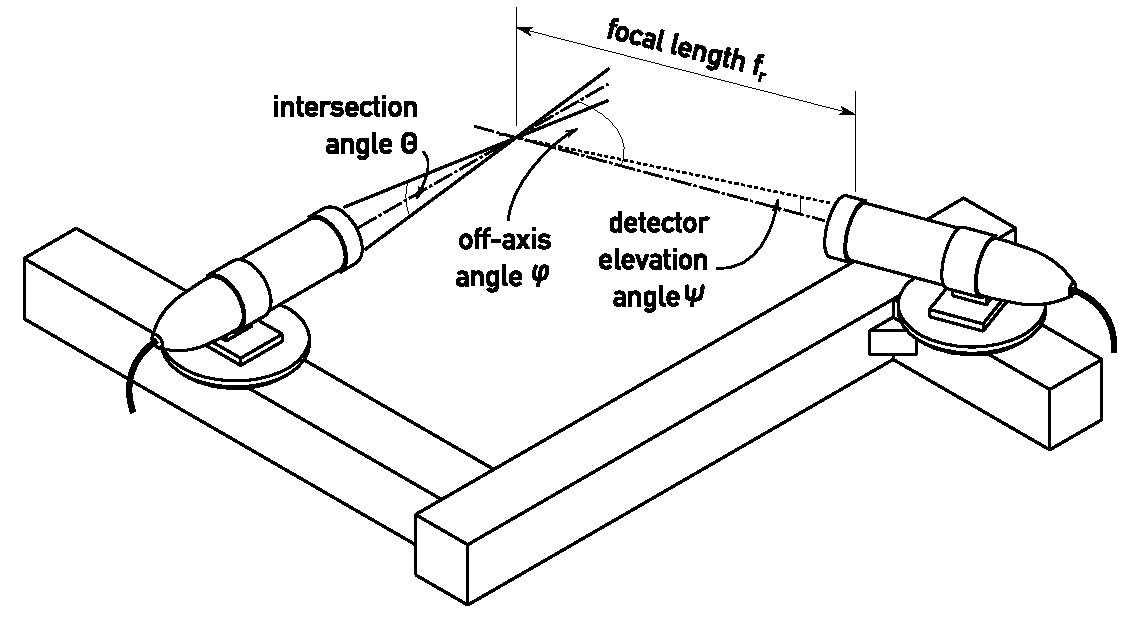
\includegraphics[width=0.75\textwidth]{img/setup/pdpa_angles.pdf}
    \caption{Nomenclature used for the geometry in \figref{fig:pdpa-setup} \label{fig:pdpa-angles}}
\end{figure}

\subsection{Large particles}
In practice, we do not deal with droplets smaller than tens of microns (much
less sub-micron particles, to which the above would apply). We therefore apply a
somewhat more complex model, in which the fields of both scattered beams are
considered separately. Indeed, their interference is modelled directly at the
receiver.

Depending on the the relative refractive index $m$, either the reflected light
or the light of a certain scattering order dominates when seen from an off-axis
angle $\phi$. In the setup shown in \figref{fig:pdpa-setup}, $\phi = 60^\circ$
and $m$ is assumed to be 1.33 (water droplets in air). In this setup, the
receiver will see the beams mostly as first-order refracted rays. An extensive
numerical evaluation of these relationships was published by \citet{Naqwi96}.

From the perspective of the receiver, each beam is scattered from a glare point
on the droplet surface. Due to the path length differences and the falling
motion past the receiver probe, the intensities from both glare points create a
beating frequency on both detectors, which are offset in space (on the order of
millimeters) and therefore measure the beating signal with slight phase shifts
(on the order of a few $\pi$). \figref{fig:pdpa-moire-static} illustrates how larger
droplets result in narrower fringes, and thus a larger phase difference.

Note, however, that the patterns shown in \figref{fig:pdpa-moire-static} are
valid only for stationary droplets. Falling droplets experience a Doppler
effect: the upward-angled beam is sampled at a relatively higher velocity,
leading to a higher scattered frequency. The downward-angled beam, on the other
hand, is scattered at a lowered frequency. The discrepancy in frequency leads to
curved fringes. Moreover, the direction of the receiver changes as the droplet
is falling. The result is not directly intuitive: the velocity has no impact at
all on the phase difference between detectors A and B, and the size has no
impact on the beat frequency (i.e. burst frequency) measured by the detectors.

\begin{figure}
    \centering
    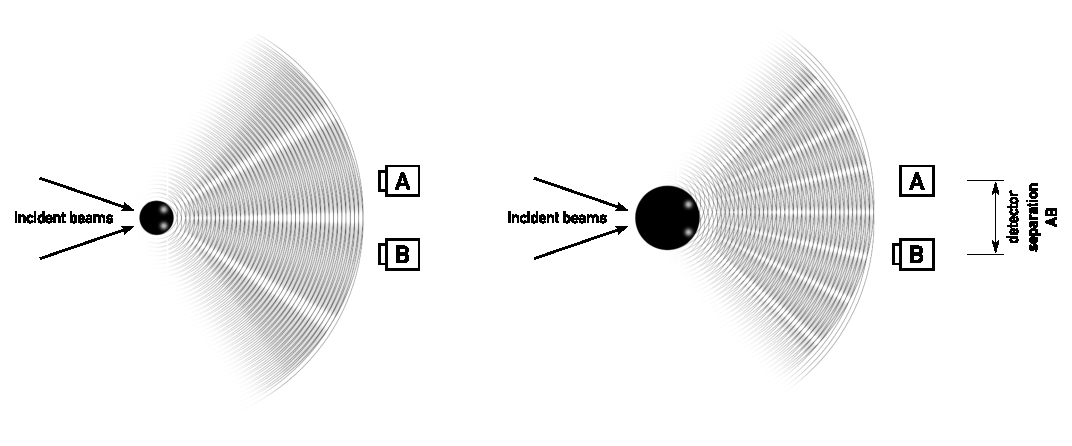
\includegraphics[width=\textwidth]{img/setup/pdpa_moire_static.pdf}
    \caption{Moiré-style visualization of the interference pattern cast by the
    two glare points. Left: glare points on small particles are close, resulting
in wide fringes. The signals recorded by detectors A and B are shifted in time
by a phase difference $\Delta \Phi_{AB}$, which is due to the detectors' known
separation in space. Right: glare points on larger particles are farther apart,
resulting in narrower fringes and a larger phase difference.
\label{fig:pdpa-moire-static}}
\end{figure}

For first-order refraction, \citet{Albrecht03} provide the following
relationship between droplet diameter $d_p$ and the difference in measured
phase $\Phi$ between two detectors A and B:
\begin{equation}
    \begin{split}
        \Delta \Phi_{AB} &= \beta_{AB} d_p \\
                         &= \frac{2\pi}{\lambda} \left(\Phi_A - \Phi_B\right) d_p \\  
                         & 
        \begin{split}
            \;=\frac{2\pi}{\lambda} d_p \Bigg[\,&\sqrt{1+m^2-\sqrt{2} m
        \sqrt{1+\sin \psi_A \sin \frac{\Theta}{2} + \cos \psi_A \cos \phi_A \cos
    \frac{\Theta}{2}}} \\
        -{} &\sqrt{1+m^2-\sqrt{2} m \sqrt{1-\sin \psi_A \sin \frac{\Theta}{2} + \cos \psi_A \cos \phi_A \cos
    \frac{\Theta}{2}}}\\
        -{}&\sqrt{1+m^2-\sqrt{2} m \sqrt{1+\sin \psi_B \sin \frac{\Theta}{2} + \cos \psi_B \cos \phi_B \cos
    \frac{\Theta}{2}}}\\
    +{}&\sqrt{1+m^2-\sqrt{2} m \sqrt{1-\sin \psi_B \sin \frac{\Theta}{2} + \cos \psi_B \cos \phi_B \cos
    \frac{\Theta}{2}}}\; \Bigg]. \label{eq:pdpa-full}
\end{split}
    \end{split}
\end{equation}
Note that \figref{fig:pdpa-angles} explains some of the notation used above.

Because of the periodic nature of the arriving signal, any phase difference value
exceeding one period ($2\pi$) is indistinguishable from one below one period.
One solution to this problem is to consider the signal bursts from both
detectors in their entirety and to determine the time shift between them (time
shift technique) \cite{Albrecht03}. Another, more commonly implemented solution
is the addition of a third detector, spaced very closely to the first. Then the
phase difference between detectors A and C is
\begin{equation}
    \Delta \Phi_{AC} = \beta_{AC} d_p.
\end{equation}
Since the slopes $\beta_{AB}$ and $\beta_{AC}$ are known, we can then deduce how
many $2\pi$ jumps should be contained in the measured $\Delta \Phi_{AB}$:
\begin{equation}
    n_{2\pi} = \mathrm{int}\left[
        \frac{1}{2\pi}\left(\frac{\beta_{AB}}{\beta_{AC}} \Delta \Phi_{AC} -
    \Delta\Phi_{AB} \right) + \frac{1}{2}\right]
\end{equation}
This allows us to bring $\Delta\Phi_{AB}$ into the range $[0, 2\pi]$:
\begin{equation}
    \Delta\Phi_{AB} = \beta_{AB} d_p - 2\pi n_{2\pi}
\end{equation}
We are now able to solve for $d_p$:
\begin{align}
    d_{p,AB} &= \frac{\Delta\Phi_{AB} + 2\pi n_{2\pi}}{\beta_{AB}}\\
    d_{p,AC} &= \frac{\Delta\Phi_{AC}}{\beta_{AC}}
\end{align}
If the discrepancy between the two values are below a set threshold, the
measurement is accepted.

\begin{figure}
    \centering
    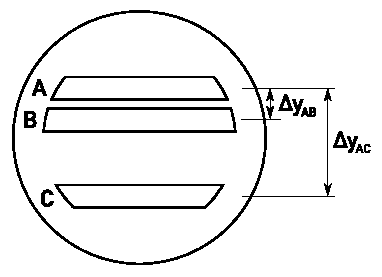
\includegraphics[width=0.5\textwidth]{img/setup/detector_arrangement.pdf}
    \caption{Typical vertical arrangement of detectors A, B, and C in a receiver
        probe. Detector separation values are indicated. \label{fig:pdpa-detector-arrangement}}
\end{figure}

Generally, the elevation angle $\psi$ of a given detector is not known. However,
it can be estimated from the detector separation values (see
\figref{fig:pdpa-detector-arrangement}) and the focal length of the receiver's
lens $f_r$.

\subsection{Calculation in TSI FlowSizer software}
To verify the results displayed by the TSI FlowSizer software, it was necessary to
understand how FlowSizer arrives at a diameter distribution from the measured
phase data. Although their algorithm is not published, it is possible to reverse
engineer their approach by deriving the required mathematical simplifications.
We then compared the results to an implementation of the full equation given
above, based on a set of raw detector phase data.

FlowSizer records the phase differences between detector pairs AB and AC,
ranging from $-180^\circ$ to $180^\circ$. We must first adjust these values to
yield strictly positive phase differences. To this end, we add $360^\circ$ to
all negative phase difference values to map them onto equivalent phositive phase
differences.

\citet{Albrecht03} then provide a simple approximation of \eqref{eq:pdpa-full}
under a number of assumptions (e.g. $\sin \psi \approx \psi$ etc.):
\begin{align}
    \Delta\Phi_{AB} &\approx -\frac{2\pi}{\lambda} d_p \sin \psi_{AB} \sin
    \frac{\Theta}{2}\frac{m}{v \sqrt{1 + m^2 - mv}}
    \label{eq:pdpa-phase-simple-ab}\\
    \Delta\Phi_{AC} &\approx -\frac{2\pi}{\lambda} d_p \sin \psi_{AC} \sin
    \frac{\Theta}{2}\frac{m}{v \sqrt{1 + m^2 - mv}}, \label{eq:pdpa-phase-simple-ac}
\end{align}
with 
\begin{align}
    v_{AB} &= \sqrt{2(1 + \cos \psi_{AB} \cos \phi \cos \frac{\Theta}{2})} \\
    v_{AC} &= \sqrt{2(1 + \cos \psi_{AC} \cos \phi \cos \frac{\Theta}{2})}
\end{align}

FlowSizer first makes the assumption that $\cos \psi_{AB} \approx \cos \psi_{AC} \approx
0.995$, and thus simply computes

\begin{equation}
    v = \sqrt{2(1 + 0.995 \cos \phi \cos \frac{\Theta}{2})}
\end{equation}

They also designate as ``slope'' (here, $\gamma$) the second term of
\eqref{eq:pdpa-phase-simple-ab} and \eqref{eq:pdpa-phase-simple-ac}:
\begin{equation}
    \gamma = \frac{m}{v \sqrt{1 + m^2 - mv}}.
\end{equation}

Also, the fringe distance at the center of the illuminated volume, given
perfect alignment, is given by \citet{Albrecht03} to be:
\begin{equation}
    \delta x = \frac{\lambda}{2 \sin \frac{\Theta}{2}}.
\end{equation}
Finally, FlowSizer appears to use the approximation 
\begin{align}
    \sin \psi_{AB} &= \frac{\Delta y_{AB}/2}{f_r} \\
    \sin \psi_{AC} &= \frac{\Delta y_{AC}/2}{f_r},
\end{align}
where $\Delta y_{AB}$ is the physical separation between detectors A and B (e.g. in
millimeters) and $f_r$ is the focal length of the receiver lens.

It follows that \eqref{eq:pdpa-phase-simple-ab} and \eqref{eq:pdpa-phase-simple-ac}, when
rewritten for $\beta$, can be composed as
\begin{align}
    \beta_{AB} &= \frac{\Delta y_{AB}}{2f_r} \gamma \frac{360^\circ}{\delta x} \\
    \beta_{AC} &= \frac{\Delta y_{AC}}{2f_r} \gamma \frac{360^\circ}{\delta x}
\end{align}
Where we write $360^\circ$ instead of $2\pi$ since FlowSizer works with phase
values in degrees. This is a useful approximation, because now $\beta_{AB}$ and
$\beta_{AC}$ only depend on constant values (including $\Delta y_{AB}$ and
$\Delta y_{AC}$, which can be set in the software).

FlowSizer then filters out all $d_{p,AB}, d_{p,AC}$ pairs that differ by more than some
threshold. The manual recommends seven percent of the maximum measureable size,
which in practice evaluates to a few tens of microns.

\subsection{Calibration in TSI FlowSizer}
It follows from the above equations that no calibration should be necessary at
all, as long as all angles and distances are well-known. However, $\Delta
y_{AB}$ and $\Delta y_{AC}$ are not typically known to great precision. The
solution, then, is to determine their values based on the phase differences
recorded after measuring monodisperse droplets of known size.

The TSI FlowSizer software provides this functionality. Presuming a vibrating
orifice droplet generator is used, flow rate and frequency can be entered and
are converted to droplet diameter using \eqref{eq:dropdia-continuous}. The
software then adjusts $\Delta y_{AB}$ and $\Delta y_{AC}$ such that the peak (if
any) or some still-unknown measure of average of the diameter distribution
aligns with the expected droplet diameter. This is easily done, since due to the
approximation of $\cos \psi \approx 0.995$, the value of $\gamma$ no longer
depends on $\Delta y_{AB}$ and $\Delta y_{AC}$ and can be set independently.


\section{Sources of error}
\subsection{Gaussian beam divergence}
The theory predicting the linear relationship between detector phase difference
and droplet diameter is founded on the assumption of very small droplets and
plane beam wavefronts. Unfortunately, when particles larger than the beam cross
the measurement volume in certain directions, glare points of the normally
dominant scattering order (e.g. first-order refraction) can temporarily become
weak enough to be dominated by another scattering order (e.g. reflection). This
phenomenon leads to erroneous results, of course, and is termed \emph{trajectory
ambiguity effect} (TAE) or \emph{Gaussian beam defect} (GBD) in the literature.

The problem was recognized first by \citet{Saffman86}, but had to be neglected until
the plane-wave scattering theory of Lorenz-Mie optics was extended into
the \emph{Generalized Lorenz-Mie Theory} (GLMT). Most of this work was
done by Gouesbet, Gréhan, Maheu, Lock and others throughout the 1980s
\cite{Grehan80, Gouesbet82, Gouesbet88, Maheu88}, and mathematically
rigorous formulations were available by the early 1990s \cite{Lock94,
Gouesbet94}. The 1996 paper by Gouesbet and Gréhan summarizes these developments
and provides an early overview over the attempts to circumvent the TAE
\cite{Gouesbet96}. 

Solutions proposed in \citet{Albrecht03} include planar setups (a different
geometry, in which detectors are placed in line with the beams) and validity
checks between the diameter determined by detector pairs AB and AC.

\subsection{Slit effect}
Most commercial phase-Doppler systems use a slit aperture in front of the
detector or receiving fibers \cite{Albrecht03}. This helps to define the
detection volume in the $z$ dimension (i.e. the beam direction), which is necessary for further statistics
about flux, and it can be useful when sprays are very dense, as multiple
droplets may be present within the measurement volume at a time.

It can occur, however, that the aperture cuts off the dominant-order glare point
of a droplet that is just halfway outside of the visible region. In that case,
the glare point corresponding to the non-dominant scattering order will
dominate and result in a wrong measurement. A graphical representation is shown
in \figref{fig:sliteffect}. 

\begin{figure}
    \centering
    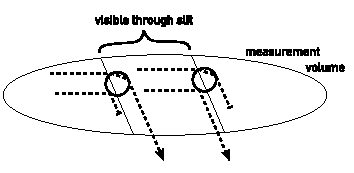
\includegraphics[width=0.5\textwidth]{img/setup/sliteffect.pdf}
    \caption{Schematic illustrating the slit effect. Two small droplets are
    passing through the measurement volume (top view; trajectories are into the
page). The droplet on the left only scatters its refracted glare point onto the
receiver (as normally intended at $\phi=60^\circ$). Refraction is suppressed,
however, for the droplet on the right; the slit aperture only allows the
reflected light to pass. \label{fig:sliteffect}}
\end{figure}

Durst et al show experimentally that the slit effect is even more crucial than
the Gaussian beam effect. \cite{Durst94}. Together with the TAE, this
is called the measurement volume effect. As with the slit effect, three-detector
setups are significantly less sensitive to this problem because of the
additional validation. Qiu and Hsu propose using four detectors, instead of
three, to resolve this problem entirely \cite{Qiu99}. A similar design was
verified experimentally by \citet{Sipperley14}.

A more recent review of the phenomenon and associated techniques was published by
\citet{Strakey00, Strakey00a}.

\subsection{Change in fringe frequency over $z$}
The sphericity of the beam wavefronts causes the fringe spacing to vary along
the major axis of the measurement volume. At the near and far ends of the
volume, the fringes are spaced farther apart, which can result in an error on
the order of 10\% according to \citet{Albrecht03}. The most important factor is
the beam waist dislocation (i.e. misalignment), which must be minimized. The
error is also reduced for wider beam waists and larger intersection angles
$\Theta$.

\subsection{Selection of lenses and masks}
\citet{Davis04} have shown that the selection of lenses and detector masks
can have a considerable effect on droplet sizing results. In their experiment,
they measured the same spray using several combinations of focal lengths and mask
sizes and found that if the diameter range to be measured is not known a priori,
it can be very difficult to choose an appropriate lens-mask combination.

\subsection{Optical aberrations}
\citet{Dressler90} investigated several error sources arising in PDPA
calibration, and found that the spherical aberration of the transmitter lens
typically gave errors of less than 3\%.

\subsection{Dirty fiber ends}
The ends of the transmitter fibers should be polished regularly. Dirty or
scratched fiber ends can mar the Gaussian beam profiles, leading to distortions
or irregularities in the measurement volume's fringe pattern.

\subsection{Wrongly entered parameters}
The optical principle involves many more geometric parameters than are needed
for the operation of ILIDS or laser diffraction (Malvern) devices. As a result, an
excellent interface and a very attentive user are required to ensure accurate
results.

In practice, I always get error messages when doing the last step, and the
values are way out of the expected range. The result, then, is that the D20 is
made very close to the expected monodisperse diameter. Since the D20 is quite
a bit larger than the actual (and completely obvious) peak value, even these
"wrong" values aren't correct.

\section{Calibration}

The calibration of 

- To calibrate, we re-calculate the AB/AC separation values such that the peak
corresponds with the known diameter. 
- The "peak" is ambiguous, but we can use Gaussian kernel density estimates to
find it
- There is no unique AB/AC pair that aligns the the peak to the known diameter;
many different pairs are possible.
- The difference-diameter plot should be as straight as possible, which
practically means that the PCA should be aligned horizontally (or vertically,
when it's very thin?). Or we could try to minimize the sum of absolute/squared
differences.
- All of this forces us to use a search algorithm. It is not clear how TSI does
it.



Calibration is tricky, because 

peakdiam = argmax(gaussian(average(diamAB[within7percent], diamAC[within7percent])))

Since the selection of droplets with <=diff(diam) and the gaussian kernel
density estimate are one-way functions, it's impossible to work backwards. We
also want to minimize the angle in the difference-diameter plot, i.e. the PCA is
supposed to be as close as possible to 0 and 90 degrees. So the only way to do
this reliably is to iterate over the two AB and AC values to find an optimum.

Nonetheless, even with this method the relationship between the distance values
AB and AC is typically linear, and once the linear relationship has been found,
we can find the combination of values that produces the most straight PCA and
the most centered cluster. Let's approximate the 

\chapter{Breakup of a water jet when colliding with an air jet}
We built an angle plate like this:
\begin{figure}
    \centering
    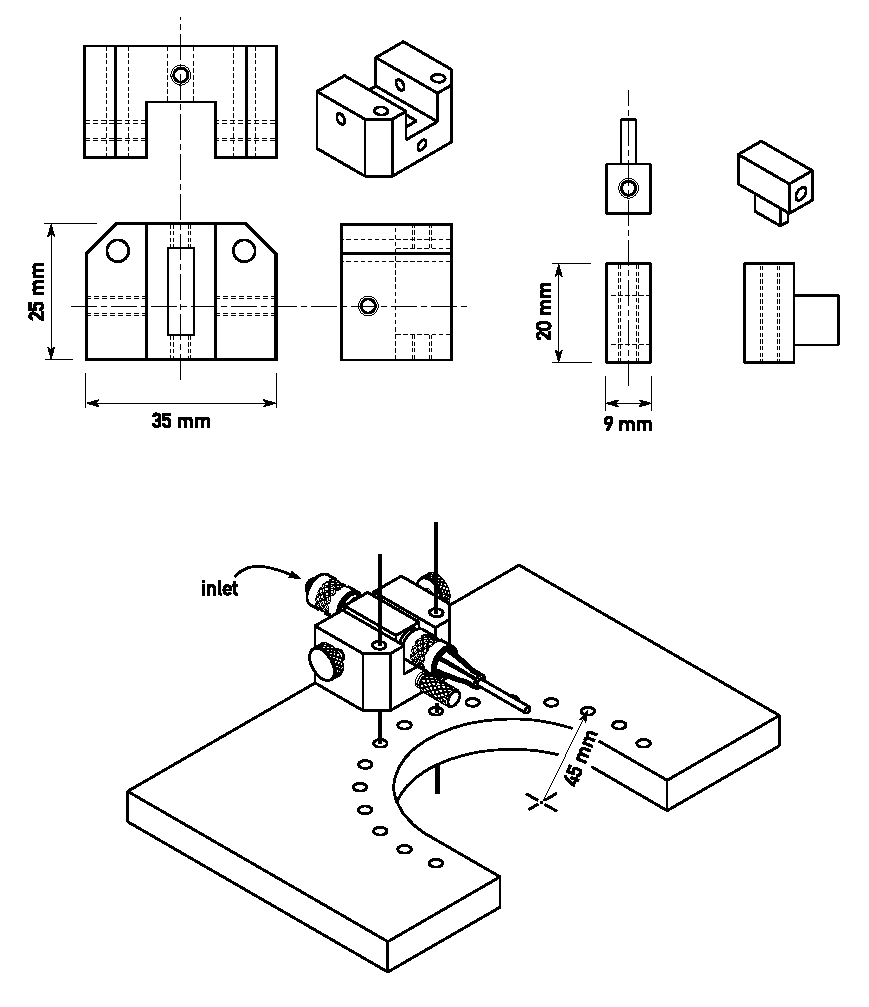
\includegraphics[width=\textwidth]{img/setup/angleplate.pdf}
    \caption{Angle plate setup}
    \label{fig:angle-plate}
\end{figure}
\bibliographystyle{myplainnat}
\bibliography{bibliography}
\end{document}
